%-------------------------------------------------------------------------------
%	PACKAGES AND OTHER DOCUMENT CONFIGURATIONS
%-------------------------------------------------------------------------------
\documentclass[a4paper, 11pt, twoside]{book}
\usepackage[brazilian]{babel}
\usepackage[utf8x]{inputenc}
\usepackage{amsmath}
\usepackage{hyperref}
\usepackage{mdframed}
\usepackage{graphicx}
\usepackage{parskip}
\usepackage{subcaption}
\usepackage{float}
\usepackage[colorinlistoftodos]{todonotes}
\usepackage[hmarginratio=3:2]{geometry}


% Defining figures base folder
\graphicspath{{figs/}}
% Resizing captions sizes
\captionsetup[figure]{font=footnotesize,labelfont={footnotesize,bf}}

% Definindo cores dos links
\hypersetup{
    colorlinks = false,
    linkbordercolor = {white},
}

% New command for importing chapters easily
\newcommand{\chapterfile}[2]{%
	\chapter{#2}%
	\label{#1}%
	\@inputTeXFile{#1}%
}

% Defines a new command for the horizontal lines, change thickness here
\newcommand{\HRule}{\rule{\linewidth}{0.5mm}}
\newcommand{\newminline}{\\[0.2cm]}


% Creating Definition environment
\newenvironment{definicao}[1]
	{
		\begin{mdframed}[topline=false,rightline=false,bottomline=false]
		\large \textsc{Definição} $\cdot$ \normalsize \textbf{#1}

	}
	{\end{mdframed}}



% Removing paragraphs
\setlength\parindent{0pt}









\begin{document}
	\frontmatter

	%-----------------------------------------------------------------------------
	%	TITLE PAGE
	%-----------------------------------------------------------------------------
	\begin{titlepage}
		% No style in cover
		\thispagestyle{empty}
		% Centraling content in page
		\newgeometry{margin=1in}
		\center

		%	HEADING SECTIONS
		\textsc{\LARGE Universidade de Brasília}\\[1.5cm] % Name of your university/college
		\textsc{\Large Notas de Aula}\\[5cm] % Major heading such as course name

		%	TITLE SECTION
		\HRule \\[0.4cm]
		{\huge \bfseries Fundamentos de Sistemas Computacionais}\\[0.4cm]
		{\Large \textsc{Sistemas Operacionais}}
		\HRule \\[6.5cm]

		%	AUTHOR SECTION
		\begin{minipage}{0.4\textwidth}
		\begin{flushleft} \large
		\emph{Autor:}\\
		Felipe \textsc{Rodopoulos} % Your name
		\end{flushleft}
		\end{minipage}
		~
		\begin{minipage}{0.4\textwidth}
		\begin{flushright} \large
		\emph{Professora:} \\
		Dr. Alba \textsc{Melo} % Supervisor's Name
		\end{flushright}
		\end{minipage}\\[2cm]

		%	DATE SECTION
		\vfill
		{\large \today}\\[2cm]
	\end{titlepage}








	%-----------------------------------------------------------------------------
	%	CONTENT
	%-----------------------------------------------------------------------------
	% Default margins for the rest of the document
	\restoregeometry

	% Index
	\tableofcontents

	% Content
	\mainmatter
	\chapter{Revisão}

\begin{definicao}{Sistema Operacional}
  Um programa ou conjunto de programas que possui duas grandes funções:
  \begin{itemize}
    \item \textbf{Criar para o usuário uma abstração do hardware}, simplificando a máquina real, escondendo a complexidade do hardware;

    \item \textbf{Gerênciar os recursos da máquina}, mantendo informações sobreo estado, endereço, controle de acesso dos mesmos, alocando e liberando-os apropriadamente, de forma eficiente e previsível.
  \end{itemize}
\end{definicao}

Note que o computador é um conjunto de recursos que serão compartilhados, onde temos:
\begin{itemize}
  \item \textbf{Recursos físicos:} processadores, memórias, discos, terminais, etc.;

  \item \textbf{Recursos abstratos:} processos, arquivos, etc..
\end{itemize}

Levando em conta a gerência de recursos, o SO deve:
\begin{itemize}
  \item \textbf{Ser eficiente:} maximizar a utilização dos recursos, ou seja, \textbf{se existe demanda, o recurso tem que estar ocupado};

  \item \textbf{Possuir um tempo de resposta previsível:} onde, preferivelmente, este tempo deve ser rápido.
\end{itemize}

% TODO: pegar imagem do Silberchatz da arquitetura do computador














\section{Estruturação de Sistemas de Computação}
\begin{definicao}{\textit{Bootstrap}}
  Programa executado quando o computador começa a funcionar, tendo como funções:
  \begin{itemize}
    \item \textbf{Inicializar o sistema}, o que inclui registradores, memória, controladores de I/O. Por exemplo, temos operações como zerar o \texttt{PC};
    \item \textbf{Verificações de hardware}, principalmente os dispositivos do computador;
    \item \textbf{Carregar o SO}. Repare que o que existir no setor 0 do disco será o programa a ser iniciado pelo \textit{bootstrap}, devendo este se o SO;
    \item \textbf{Terminar a execução}, dado que é necessário que ele mesmo termina sua execução, uma vez que ele é um microcódigo.
  \end{itemize}
\end{definicao}

Ao ligar o computador, o \textit{bootstrap} realiza checagens e rotinas iniciais, carregando o sistema operacional. O SO nunca deve terminar sua execução, a não ser quando é instruído para tal ou quando ocorre \textbf{panic}.

Após ser iniciado, o SO inicia outros processos como o \textbf{init} e outros que rodam em background, chamados \textbf{daemons}. Depois disso, ele apenas aguarda a ocorrência de eventos, os quais são sinalizados por interrupções.


















\section{Interrupções}
Interrupções podem ser tanto de \textit{hardware} como de \textit{software}.

Interrupções de \textit{harware} são sinais enviados para a CPU através de barramentos.

Interrupções de \textit{software} são geradas por operações especiais conhecidas como \textbf{chamadas de sistema (\textit{system calls})}. Podemos chamá-las de \textit{monitor calls} ou \textit{supervisor calls}, sendo essas nomenclaturas arcaicas.

A interação entre o sistema operacional e os programas é através de chamadas de sistema.



\subsection{Tratamento de Interrupções}

Este processo \textbf{envolve tanto hardware como o sistema operacional}. Quando ocorre uma interrupção, temos os seguintes passos:
\begin{enumerate}
  \item O hardware interrompe a execução corrente e salva seu estado na pilha, o que inclui registradores, descritores, etc.;

  % TODO: o PC é apontado para o endereço do Vetor de Int.?
  \item O hardware acessa um endereço específico de memória física, onde há o \textbf{vetor de interrupções}. Nele, os endereços das rotinas de tratamento de interrupções geradas por cada dispositivo está contido;

  \item O sistema operacional executa o tratamento de interrupção indicado. Os registradores que foram empilhados pelo hardware são salvos em memória;

  \item A interrupção é devidamente tratada;

  \item A CPU volta à execução anterior à ocorrência da interrupção.
\end{enumerate}

\begin{definicao}{Vetor de Interrupções}
  Contém o endereço da rotina de tratamento de interrupções, geradas por cada classe de dispositivo físico: disco, flop, terminal, etc..
\end{definicao}


\textbf{Nota:} a rotina de tratamento de interrupção e seus endereços contidos no vetor de interrupções são gerados e escritos pelo sistema operacional.



















\section{Modos do Processador}

Determinam a abrangência da execução de um programa em um computador. Temos dois:

\begin{itemize}
  \item \textbf{Modo Protegido (\textit{Kernel}):} o processador pode executar qualquer instrução do seu conjunto de instruções.

  \underline{Exemplos:} instruções de I/O, instruções que alteram o estado de execução; \\

  \item \textbf{Modo Usuário:} apenas um subconjunto definido de instruções pode ser executado.
\end{itemize}

A \textbf{instrução de trap} seta o bit de modo usuário para o modo protegido e desvia a execução para instruções localizadas no espaço do sistema operacional.

\begin{definicao}{\textit{Kernel}}
  Parte do sistema operacional que se executa em modo protegido.
\end{definicao}













\section{Entrada e Saída}
Alguns dispositivos não possuem suporte a interrupções e logo necessitam usar o \textit{polling}.

\begin{definicao}{\textit{Polling}}
  Esquema de entrada e saída, onde o dispositivo de I/O sinaliza uma interrupção ao setar um \textit{flag} em um registrador específico, periódicamente consultado pelo SO.
\end{definicao}


Além disso, podemos ter dois esquemas de entrada e saída:
\begin{itemize}
  \item \textbf{Síncrono:}
% TODO: fazer aqui
  \item \textbf{Assíncrono:}
\end{itemize}

A \textbf{tabela de dispositivos} será a estrutura que irá auxiliar no acompanhamento dos estados de cada dispositivo de I/O que está esperando ser atendido.






















\section{Direct Memory Access}
Quando a controladora lê dados de um dispositivo, estes são armazenados inicialmente em um \textit{buffer} interno. Estando o bloco completo e correto neste buffer, o mesmo deve ser escrito em memória.

% TODO: a escrita então é exclusiva da controladora? Ou isso varia de arquitetura para arquitetura
Esta escrita em memória não pode ser feita pela CPU, pois iria esta operação consome muito tempo, dadas as operações de cópia. Desta forma, normalmente, a operação acaba ficando a cargo da controladora, através de operações de acesso direto à memória, ou DMA. Este processo ocorre através das seguintes etapas:

\begin{enumerate}
  \item O SO informa o endereço de memória para o qual o dado deve ser lido e o número de \textit{bytes} a serem transferidos;

  \item As informações são escritas pela controladora em dois registradores DMA, onde um é de endereço e o outro o contador;

  \item A controladora lê o bloco do dispositivo de I/O;

  \item Após ter o bloco completo em seu buffer, a controladora transfere o conteúdo de ser buffer - \textit{byte} a \textit{byte} - para o endereço de memória especificado no registrador DMA;

  \item Quando o contador chega a zero, a controladora gera uma interrupção;

  \item O SO inicia a execução sabendo que o bloco já se encontra no endereço de memória destino.

\end{enumerate}























\section {Estrutura dos Sistemas Operacionais}

\subsection{Sistemas Monolíticos}
Organização de SOs mais comum, onde \textbf{não há estrutura, sendo o SO um conjunto de procedimentos que chamam um ao outro}. O SO roda em modo \textbf{kernel} enquanto os demais programas rodam em modo usuário.
\underline{Exemplos:} Unix comercial.

Pode-se obter um mínimo de estruturação se os procedimentos são forçados à fazer \textit{syscalls}, gerando \textit{traps}. Ou seja, o próprio sistema operacional chama a si mesmo, para confinar o erro na rotina de tratamento.

Geralmente, essas arquiteturas possuem três camadas conceituais, dado que é possível burlá-las. Elas são:
\begin{itemize}
  \item \textbf{Procedimento principal}, que chama os de serviço;
  \item \textbf{Procedimento de serviços}, que tratam as chamadas ao sistema;
  \item \textbf{Procedimentos auxiliares}, que ajudam os procedimentos de serviço.
\end{itemize}

\begin{figure}[ht]
  \centering
  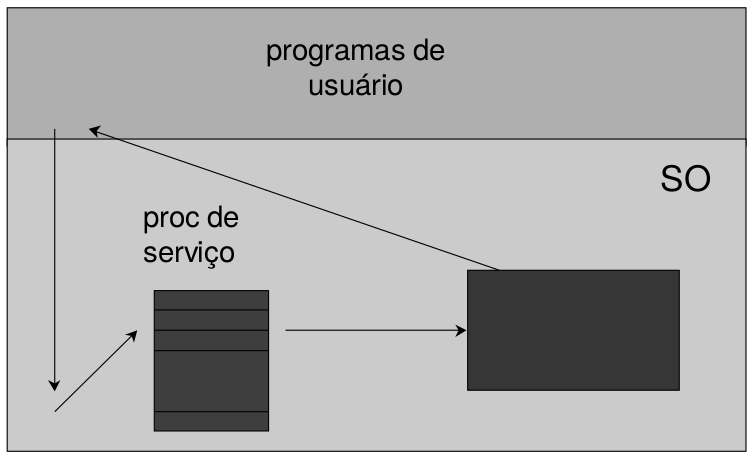
\includegraphics[width=0.75\textwidth]{os-arch-mono}
  \caption{Sistema operacional com arquitetura monolítica}
  \label{fig:os-arch-mono}
\end{figure}

\textsc{Vantagens}
\begin{itemize}
  \item A falta de estrutura acaba melhorando a performance do sistema e, por isso, \textbf{esta é a organização mais eficaz, em termos de tempo de resposta}.
\end{itemize}

\textsc{Desvantagens}
\begin{itemize}
  \item Não oferece uma boa manuntenção de código;
\end{itemize}







\subsection{Sistemas em Camadas}
Nesta organização, cada camada só interage com suas camadas adjacentes, sendo esta noção fortemente reforçada pelo hardware.
\underline{Exemplos:} THE (1968 - Djikstra), MULTICS (BELL, MIT)

% TODO: Isso vale para todos as arquiteturas? Posso generalizar isso?
As camadas destinadas aos recursos da máquina ficam em modo protegido, enquanto a camada de programas de usuário fica em modo usuário.

\begin{figure}[ht]
  \centering
  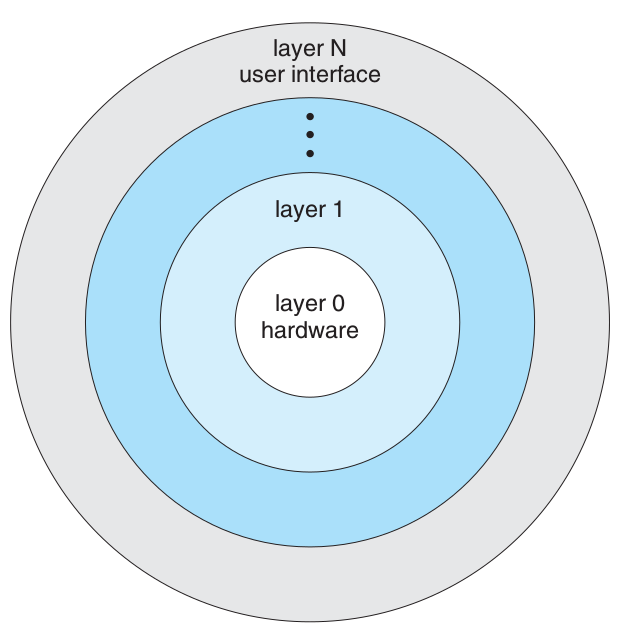
\includegraphics[width=0.65\textwidth]{os-arch-layer}
  \caption{Sistema operacional com arquitetura em camadas}
  \label{fig:os-arch-layer}
\end{figure}

\textsc{Vantagens}
\begin{itemize}
  \item Usando as camadas como forma de separar o código, acaba por oferecer melhor manutenção.
\end{itemize}

\textsc{Desvantagens}
\begin{itemize}
  \item Se o programa de usuário deseja fazer uma operação que é atribuída a uma camada na posição $n$, as $n-1$ camadas devem ser percorridas, logo há um maior \textit{overhead}. A Figura \ref{fig:os-arch-layer} retrata bem esta situação.
\end{itemize}


% TODO: usar imagem do slide SISTEMA EM CAMADAS e falar que ela é do MULTICS, LEGENDA: roxo (modo usuario) e verde (modo protegido). toda entrada e saida é feita em memória virtual; 2. se o programa do usuário quer alocar memória, conceitualmente ele deve passar pela camada de entrada e saída.







\subsection{Máquina Virtual}
Sistemas operacionais estruturados como máquina virtual possuem, no mais baixo nível, um monitor da máquina virtual, que simplesmente implementa a multiprogramação entre sistemas operacionais. Em cima do monitor, várias máquinas virtuais podem ser utilizadas.
\underline{Exemplo:} VM/370 da IBM

As máquinas virtuais implementam um cópia fiel do hardware, com modo kernel/usuário, I/O e interrupções. Quando a máquina virtual é selecionada para execução, ela assume o \textit{hardware}. Eventualmente, o monitor assume o \textit{hardware} para continuar a execução do SO e selecionar alguma outra máquina.

% TODO: legenda da imagem: quando o monitor define que uma VM vai executar, ela assume o hardware. Eventualmente, o monitor assume o hardware novamente para continuar a sua execução e de demais máquinas.

\begin{figure}[ht]
  \centering
  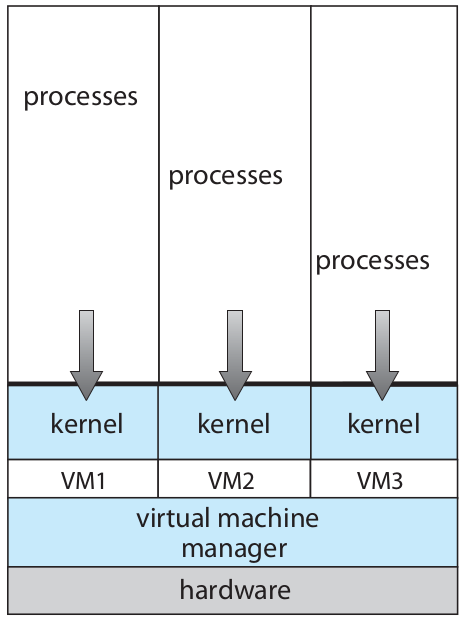
\includegraphics[height=7cm]{os-arch-vm}
  \caption{Sistema opercional com arquitetura de máquinas virtuais}
  \label{fig:os-arch-vm}
\end{figure}



\textsc{Vantagens}
\begin{itemize}
  \item Permite a utilização de mais um sistema operacional sob um mesmo \textit{hardware};
\end{itemize}

\textsc{Desvantagens}
\begin{itemize}
  \item Cria um óbvio \textit{overhead}.
\end{itemize}






\subsection{Modelo Cliente/Servidor}
Aqui, grande parte das funções do SO é implementada a nível de usuário, em forma de processos clientes. Apenas o \textit{kernel} roda em modo protegido.
\underline{Exemplo:} micro-kernels.

O \textit{kernel} funciona como um servidor para estes processos, realizando a comunicação entre eles, implementando suas abstrações. A interação entre processos ocorre por troca de mensagens, onde existem apenas duas chamadas de sistema: \textit{read} e \textit{send}.

\begin{figure}[ht]
  \centering
  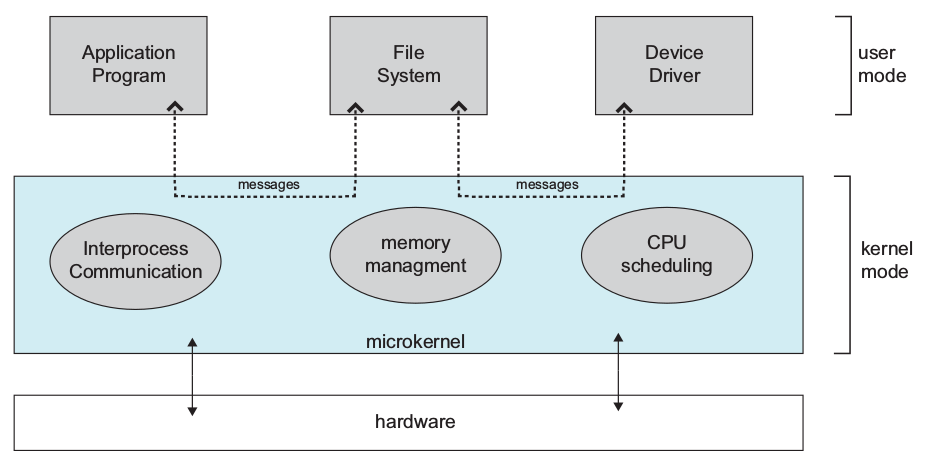
\includegraphics[width=0.75\textwidth]{os-arch-cliserv}
  \caption{Sistema operacional com arquitetura cliente/servidor. O processo cliente manda uma mensagem para o \textit{kernel}, pedindo um \textit{read} de um arquivo. O kernel envia a operação ao processo responsável, no caso o \textit{filesystem}. Este, necessita de ler do disco, logo precisa de enviar uma mensagem para o servidor \textit{driver} do mesmo. Ao fim, o caminho inverso também deve ser feito.}
  \label{fig:os-arch-cliserv}
\end{figure}

\textsc{Vantagens}
\begin{itemize}
  \item Projeto do SO acaba por ficar mais simples;
  \item O SO fica mais confiável, dado que o \textit{panic} em um processo fica retido no processo de origem e não no \textit{kernel};
\end{itemize}

\textsc{Desvantagens}
\begin{itemize}
  % TODO: ver se isso esta correto e destrinchar. Usar a imagem abaixo.
  \item As constantes trocas entre modo usuário e modo protegido acabam por gerar um custoso \textit{overhead}, fazendo esta ser a arquitetura com menor desempenho entre as quatro;
\end{itemize}


% TODO: legenda para a figura.

	\chapter{Processos}

\begin{definicao}{Processo}
  É um programa em execução, composto por:
  \begin{itemize}
    \item Código em execução;
    \item Pilha de execução e seu apontador;
    \item Contado de programa (\texttt{PC});
    \item Valores de registradores de máquina;
    \item E outras informações.
  \end{itemize}
\end{definicao}

Cada processo possui um identificador único, conhecido como \textit{pid}. As informações do processo ficam armazenadas na \textbf{tabela de processos}, sendo o \textit{pid} seu indexador na tabela.

Durante a execução, o processo compartilha o processador com outros processos, sendo eles escalonados ao longo do tempo. A interação entre processos ocorre por mecanismos de comunicação próprios.

Por fim, existem dois escopos que carregam variáveis sobre a execução do processo:

\begin{itemize}
  \item \textbf{Ambiente:} contendo o espaço de endereçamento, arquivos abertos, processos filhos, sinais, estatísticas de uso, etc.;

  \item \textbf{Execução:} contendo registradores utilizados pelo processo, como o PC e o apontador de pilha, e o estado de execução do processo.
\end{itemize}

\begin{figure}
  \centering
  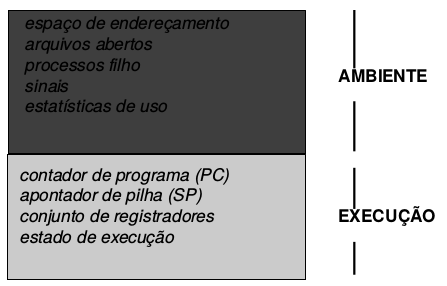
\includegraphics[width=.5\textwidth]{process-model}
  \caption{Modelo padrão de escopo de um processo}
  \label{fig:process-model}
\end{figure}
















\section{Modelo de Processos}
Classificamos os processos em relação ao custo de troca de contexto e manutenção:

\begin{itemize}
  \item \textbf{\textit{Heavyweight}:} são os processos tradicionais. Na sua entrada da tabela de processos temos tanto as informações de ambiente como as de execução;
  \item \textbf{\textit{Lightweight}:} são as \textit{threads}. Sua entrada na tabela de processos só contém informações de ambiente.
\end{itemize}

No modelo \textit{heavyweight}, também chamado de modelo tradicional, cada processo tem um único fluxo de controle, ou seja, em um dado momento ele só tem um valor de \texttt{PC}. Este processo roda independente dos demais e pode conter processos \textit{threads} que dependem dele.

Todo sistema operacional deve possuir mecanismos que permitam a criação de processos. Geralmente, um processo somente é criado por outro processo, o que nos leva uma \textbf{hierarquia de árvore de processos} (Figura \ref{fig:process-tree}). Entretanto, é necessário frisar que a árvore de processos não é de fato implementada. A partir do campo de ID do processo pai (PPID), podemos virtualmente implementar essa árvore. Implementá-la de fato seria muito custoso.

\begin{figure}[h]
  \centering
  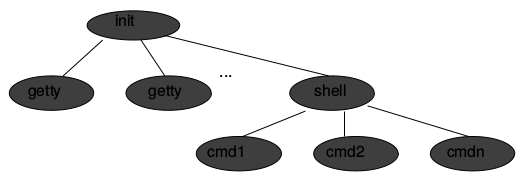
\includegraphics[width=0.6\textwidth]{process-tree}
  \caption{Esquema de uma árvore de processos padrão}
  \label{fig:process-tree}
\end{figure}




















\section{Estado do Processo}
Apesar de processos serem relativamente auto-suficientes, muitas vezes eles necessitam de acessar outros recursos (discos, terminais) ou mesmo se comunicar com outros processos. Quando um processo está ocioso, esperando que um evento aconteça, nós dizemos que ele está bloqueado. Em algumas situações, o processo pode ser bloqueado a revelia pelo sistema operacional. Podemos ter os seguintes estados:

Estados:
\begin{itemize}
  \item \textbf{Rodando:} processo em execução
  \item \textbf{Bloqueado:} processo parado, aguardando alguma coisa;
  \item \textbf{Pronto:} processo parado, pronto para ser executado, aguardando sua vez.
\end{itemize}

Usando a Figura \ref{fig:proc-states} como referências, podemos ilustrar as diversas passagens de estados ao longo da vida de um processo:

\begin{enumerate}
  \item O processo bloqueia-se à espera de um evento ou recurso;

  \item O evento ou recurso esperado pelo processo está disponível.Ele agora pode se executar, passando para o estado de \textit{Pronto};

  \item O processo é escolhido pelo escalonador para execução;

  \item O tempo de posse do processador pelo processo acabou. O SO retira o processador do processo.
\end{enumerate}

\begin{figure}[ht]
  \centering
  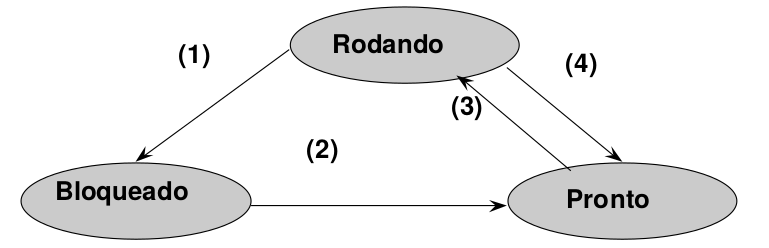
\includegraphics[width=.75\textwidth]{proc-states}
  \caption{Possíveis estados de um processo.}
  \label{fig:proc-states}
\end{figure}

















\section{Tabela de Processos}
\begin{definicao}{Tabela de Processos}
  Estrutura que contem os todas as informções relativas à manutenção de cada processo do SO, guardando os campos de gerência de processos, memória e arquivos. Possui uma entrada para cada processo.
\end{definicao}

Em relação a \textbf{gerência de processos}, as informações guardadas normalmente são: \textit{pid}, valor dos registradores de execução e PC, valor da palavra de estado, valor do apontador de pilha, estado do processo, instante do início do processo, tempo de processador utilizado e outros.

Em relação a \textbf{gerência de memória}, são guardados o endereço do segmento de texto, dados e pilha, sendo estes mandatórios. Podemos ter também estado da saída, informações sobre proteção e outros. Note que o segmento de texto é a porção de código do processo, que normalmente é \textit{read only}. Alguns sistemas com área de memória pequena tornam essa área \textit{read-write}, para uso eficiênte da memória, porém essa estratégia oferece riscos de segurança.

Em relação a \textbf{gerência de arquivos}, são guardados o diretório raíz e de trabalho, descritores de arquivos abertos, parâmetros de chamadas em andamentos e outras.




\subsection{Troca de Contexto}
\begin{definicao}{Contexto}
  No que diz respeito a processos, o contexto será o conjunto de valores dos registradores do processo.
\end{definicao}

Dessa forma, define-se a troca de contexto como a operação de salvamento dos registradores de um processo, para restauração dos conjunto de registradores de outro processo. Tal operação permite que haja a efetiva troca de processos no processador.




















\section{Escalonamento de Processos}
O algoritmo de escalonamento de processos é o responsável pela determinação de que processo, dentro do conjunto de processos prontos, vai rodar e por quanto tempo. Quando um processo solicita operações blocantes, sua execução fica suspensa até que o evento solicitado ocorra.

\textbf{Nota:} podemos citar como operações blocantes requisições ao disco, memória, entrada e saída, entre outras.

Para garantir um bom algoritmo de escalonamento, alguns \textbf{critérios} devem ser seguidos:
\begin{itemize}
  \item \textbf{\textit{Fairness}:} garantir que todos os processos do sistema terão chances de uso do processador, ou seja, \textbf{não há \textit{starvation}}. Garantir que os processos tenham chances \textit{iguais}, é algo muito forte e não usamos essa definição;

  \item \textbf{Eficiência:} se há demanda, a CPU deve estar ocupada;

  \item \textbf{Minimizar o tempo de resposta:} o tempo total decorrido até que um processo produza uma resposta ao usuário/sistema;

  \item \textbf{Minimizar o \textit{waiting time}:} ou seja, o tempo de resposta entre os estados \textit{Ready} e \textit{Running};

  \item \textbf{Maximizar o \textit{thoughtput}:} aumentar o número de processos conclúidos em um determinado tempo.
\end{itemize}

\begin{definicao}{Preempção}
  Suspensão temporária da execução de um processo.
\end{definicao}

Podemos classificar escalonadores segundo sua preempção:

\begin{itemize}
  \item \textbf{Escalonadores não-preemptivos:} quando um processo obtém o processador, ele roda até o seu fim ou até que ele peça uma operação blocante.

  Isto simplifica o projeto do escalonador, porém permite que o processo detenha a CPU por tempo arbitrário, levando-o ao monopólio do processador. Isto acaba por violar todos os critérios de um bom escalonador;

  \item \textbf{Escalonadores preemptivos:} cada processo possui um tempo máximo de permanência, chamado \textbf{\textit{quantum}}, de posse do processador. Quando o \textit{quantum} termina, o SO retira o processador deste processo, para permitir a execução de outro processo.

  Desta forma, estes escalonadores garantem um uso mais balanceado da CPU, o que levam a eles serem usados na maioria dos SOs. Entretanto, seu projeto é consideravelmente mais complexo, uma vez que os processos devem proteger suas regiões críticas de outros processos concorrentes.
\end{itemize}

\begin{definicao}{Região Crítica}
  Área que contém as estrutura de dados importantes de um processo em execução, não podendo ser acessada por concorrentemente, mas sim atômicamente.
\end{definicao}

O tempo de execução do processo é controlado por um \textit{clock} que gera interrupções em uma determinada frequência, chamadas de \textit{clock tick}. Tal ferramenta está presente em qualquer processador moderno.

O SO mantem um contador que é decrementado a cada \textit{clock tick}. Quando este contador chega a zero, o tempo de permanência do processo acabou e ele será retirado do processador. O valor inicial deste contador corresponde ao tempo máximo de permanência do processo com a CPU, denominado, \textbf{\textit{time slice}}.

Dado isto, podemos listar as \textbf{políticas de algoritmos de escalonamento} existentes.



\subsection{\textit{First Come First Served}}
Os processos que solicitam a CPU são colocados em uma fila \textit{ready}, gerênciada segundo a política FCFS: o primeiro processo que entrar, será o primeiro a ser executado por completo. Desta forma, é importante notar que este algoritmo é \textbf{não-preemptivo}.

\begin{figure}
  \centering
  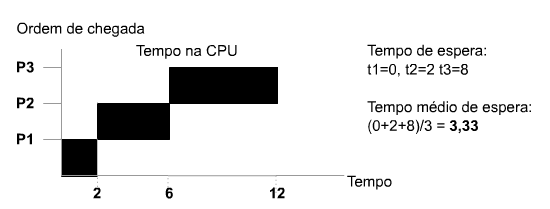
\includegraphics[width=0.75\textwidth]{scale-fcfs}
  \caption{Execução de processos em política FSFC com ordem chegada P1, P2 e P3.}
  \label{fig:scale-fcfs}
\end{figure}





\subsection{\textit{Round Robin}}
Cada processo tem o direito de usar o processador por um intervalo de tempo pré-definido, denominado \textbf{\textit{quantum}}. Quando este intervalo se esgota, o processador é dado a outro processo e o processo retirado vai para o fim da fila de processos. É versão preemptiva da política FSFC, sendo um algoritmo justo.

% TODO: colocar figura



\subsection{Escalonamento com Prioridades}
Baseia-se no fato de que alguns processos são prioritários e, assim, devem ser executados antes dos outros. A cada processo é atribuída uma prioridade e os que tem maior prioridade são executados primeiro.

A prioridade pode ser definida de duas formas:
\begin{itemize}
  \item \textbf{Estaticamente:} os processos são divididos em classes e a cada classe é atribuída uma prioridade. A cada prioridade, existe uma fila de prontos associada. A política nas filas pode ser arbitrária;

  \item \textbf{Dinâmicamente:} o sistema analisa o comportamento dos processose atribui prioridades favorecendo um certo tipo de comportamento. Por exemplo, processos com I/O podem ter prioridades altas. O cálculo da prioridade pode ser dado por $1/f$, onde $f$ é a fração do \textit{quantum} de tempo utilizado na última rodada do processo.
\end{itemize}

 Note que é possível que um processo pode monopolizar a CPU caso ele precise de muito tempo de processamento e sua prioridade for a maior de todas. A técnica de prioridade dinâmica tenta justamente mitigar este comportamento.

% TODO: colocar figura




\subsection{\textit{Shortest Job First}}
Aqui, dado um conjunto de \textit{jobs} prontos, executamos os \textit{jobs} com menor tempo de execução antes.

Note que este algoritmo pode não ser muito justo, pois, supondo um processo com uma dada prioridade, este pode entrar em \textit{starvation} se todo novo processo que entrar na fila tiver tempo de execução menor que ele.

% TODO: colocar figura





















\section{\textit{Threads}}
\textit{Threads}, ou linhas de controle múltiplas, foram criadas visando maior concorrência na execução de processos. Nelas, o processo é dividido em dois: processo em si, correspondendo ao ambiente, e a \textit{thread}, correspondendo a execução.

Um processo pode ser composto por várias \textit{threads}, onde uma \textit{thread} pode se bloquear a espera de um recurso e outra, do mesmo processo ou não, pode se executar, paralelamente. A entidade que realmente executa é a \textit{thread}, sendo o processo apenas o ambiente.

\begin{figure}
  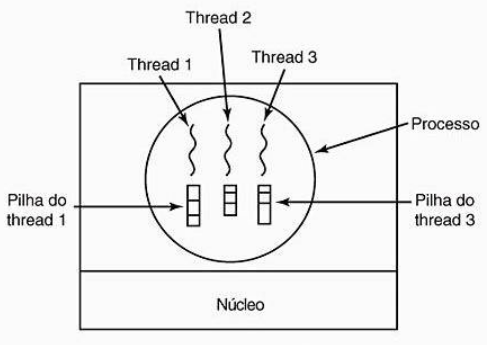
\includegraphics{threads}
  \caption{Um processo com 3 \textit{threads}, cada uma com sua pilha de execução}
  \label{fig:threads}
\end{figure}

Aqui, \textbf{a troca de contexto é mais leve}, dado que esta troca entre \textit{threads} de um mesmo processo só diz respeito a execução e não ao ambiente. Frisamos que \textbf{\textit{threads} guardam apenas o contexto de execução e não de ambiente}.

Dado isto, estas \textit{threads} compartilham as mesmas variáveis globais, memória, descritores de arquivo e outros recursos. Logo, são necessários mecanismos de \textbf{sincronização} destes recursos: variáveis \textit{mutex} e variáveis de condição.

Podemos ter dois tipos de \textit{threads}:
\begin{itemize}
  \item \textbf{Estáticas:} o número de linhas de controle que irão compor o processo é definido em tempo de compilação, fazendo com que a execução comece com o número determinado;

  \item \textbf{Dinâmicas:} as \textit{threads} são criadas e destruidas dinâmicamente, ao longo da execução do processo, criadas com primitivas específicas. A execução começa com uma \textit{thread} apontando para o início da rotina \textit{main}. Esta técnica é a mais comum.
\end{itemize}






\subsection{Implementação}
É possível implementar \textit{threads} de duas maneiras. A primeira é a \textbf{nível de \textit{kernel}}. Aqui, as abstrações de processo e \textit{threads} são implementadas pelo sistema operacional, de maneira protegida. Logo, existe a tabela de processos e uma tabela de \textit{thread} para cada processo. Isto garante um alto grau de concorrência, porém o custo da troca de contexto entre \textit{threads} continua alto, pois esta gera trocas de contexto entre modo protegido e usuário, o que é um \textit{overhead} custoso.

A segunda forma é a implementação a \textbf{nível de usuário}, simulando as \textit{threads} através de bibliotecas. Dessa forma, o custo da troca de contexto é baixo, porém quando uma \textit{thread} realizar uma operação blocante, o seu processo inteiro será bloqueado e, consequentemente, todas as suas \textit{threads-irmãs}.







\section{\textit{Deadlock}}
\begin{definicao}{\textit{Deadlock}}
  Um conjunto de processos está em \textit{deadlock} se cada processo pertencente ao conjunto estiver esperando por um evento que somente um outro processo pertencente ao mesmo conjunto pode fazer ocorrer. Como todos estão ocupados, nenhum pode provocar a ocorrência de eventos. Logo, \textbf{é uma espera eterna por recursos}.
\end{definicao}

\begin{figure}[ht]
  \centering
  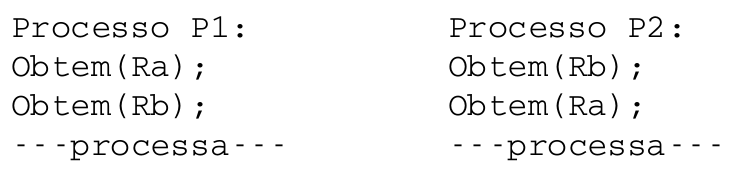
\includegraphics[width=0.7\textwidth]{deadlock}
  \caption{Uma situação clássica de \textit{deadlock}. P1 obtém \texttt{Ra}, e logo pede \texttt{Rb}. Entretanto, \texttt{Rb} está sob posse de P2, logo P1 bloqueia. Por sua vez, P2 está bloqueado, aguardando \texttt{Ra}. Logo, ambos estão bloqueados, aguardando recursos ocupados}
  \label{fig:deadlock}
\end{figure}

\begin{definicao}{\textit{Livelock}}
  Ocorre quando um conjunto de processos tentam acessar um recurso por meio de \textit{polling}, sempre encontrando esse recurso ocupado, pois estes estão alocados a processos que fazem parte do mesmo conjunto. Dessa forma, estes processos bloqueiam-se mutuamente. Logo, \textbf{há uma espera circular dentro do conjunto de processos}.
\end{definicao}

\begin{definicao}{\textit{Polling}}
  Técnica onde verifica-se periodicamente o estado de um recurso.
\end{definicao}

\begin{figure}[ht]
  \centering
  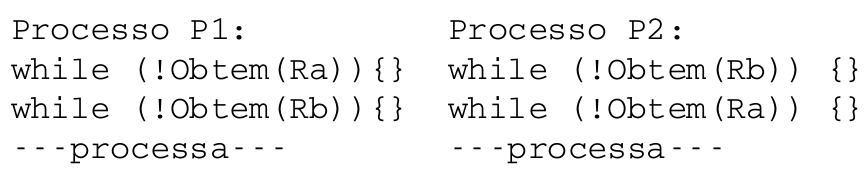
\includegraphics[width=0.7\textwidth]{livelock}
  \caption{Uma situação clássica de \textit{livelock}. A situação é análoga a da Figura \ref{fig:deadlock}, onde há um \textit{deadlock}. Entretanto, ao invés de se bloquear, os processos fazem \textit{polling} eterno.}
  \label{fig:livelock}
\end{figure}

\textbf{Nota:} Do ponto de vista teórico, \textit{livelock} e \textit{deadlock} tem significados equivalentes.

\begin{definicao}{\textit{Starvation}}
  Ocorre quando um conjunto de processos é indefinidamente preterido porque sua prioridade é menor que a prioridade de outros conjuntos de processos. Ou seja, é \textbf{uma espera por um tempo indefinido por recursos}.
\end{definicao}










\section{Comunicação entre Processos}
Processos interagem entre si, trocando informações, o que pode ser feito de duas formas: compartilhamento de variáveis ou troca de mensagens.


\subsection{Compartilhamento de Variáveis}
Nesta técnica, um processo escreve um valor em uma posição de memória e outro processo lê este mesmo valor.

Entretanto, a ordem e o tempo de execução dos processos não é previsível, dada a política de escalonamento do SO. Com isso, algumas incosistências podem ocorrer nestas áreas de memória compartilhadas, resultando em \textbf{condições de corrida}.

\begin{figure}
  \centering
  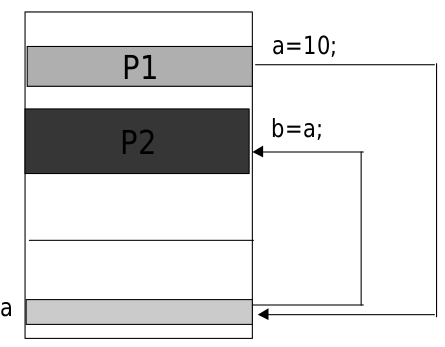
\includegraphics[width=0.5\textwidth]{variable-sharing}
  \caption{Processos $P1$ e $P2$ compartilhando a mesma posição $a$ de memória}
  \label{fig:variable-sharing}
\end{figure}

\begin{definicao}{Condição de Corrida}
  Quando dois ou mais processos acessam concorrentemente as mesmas posições de memória e o valor final contido nestas posições \textbf{depende da ordem} na qual os processos foram executados, então temos uma condição de corrida.
\end{definicao}

A condição de corrida pode não ser um erro ou algo indesejável. Alguns programadores podem tirar proveito disso. Além disso, podemos definir que os processos escrevam na mesma posição, porém forçando ser o mesmo valor. Neste último caso, \textit{não temos condição de corrida}. Porém, na maioria dos casos, é desejável eliminar as condições de corrida.





\subsection{Exclusão Mútua}
Garantir que processos ou \textit{threads} executem de forma ordenada, acessando seções críticas de maneira exclusiva é uma forma de garantir a \textbf{exclusão mútua}.

\begin{definicao}{Seção Crítica}
  Recurso ou parte do código protegida por mecanismos de exclusão mútua.
\end{definicao}

Para garantir uma exclusão mútua eficiente, a solução deve levar em contra os seguintes requisitos:
\begin{itemize}
  \item \textbf{Exclusão mútua:} a solução não pode permitir que dois processos acessem a seção crítica simultaneamente;

  \item \textbf{Progresso:} se a seção crítica está vazia e existem processos querendo acessá-la, apenas estes processos devem participar da decisão de quem vai acessá-la. Ou seja, \textbf{nenhum processo executando fora de sua seção crítica pode bloquear outros processos}.

  \item \textbf{Espera limitada:} deve existir um limite no número de vezes que outros processos acessam a seção crítica quando um processo está esperando por ela. Ou seja, \textbf{nenhum processo deve esperar eternamente para entrar em sua seção crítica}.
\end{itemize}

\textbf{Nota:} é importante frisar que levamos em conta que o programador seja correto em sua implementação, ou seja, que ele irá utilizar corretamente as ferramentas. Logo, não podemos supor que ele esqueça de indicar no programa que o processo deve sair da seção crítica.




\subsection{Exclusão Mútua com Inibição de Interrupções}
Quando um processo deseja acessar a seção crítica, o mesmo inibe todas as interrupções do SO, inibindo o escalonador de emitir interrupções para realocar a CPU. Logo, demais processos não serão executados e apenas o processo inibidor executa. Ao fim do seu acesso à seção crítica, o processo executante reabilita as interrupções. A Figura \ref{fig:syscall-inibition} dá um exemplo.

\begin{figure}[ht]
  \centering
  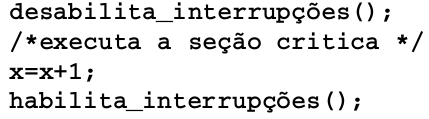
\includegraphics[width=0.5\textwidth]{syscall-inibition}
  \caption{Exemplo de código fonte para acesso à seção crítica, inibindo interrupções}
  \label{fig:syscall-inibition}
\end{figure}

Esta técnica trivialmente \textbf{preserva a exclusão mútua, a espera limitada e o progresso}, dado que apenas um processo apenas executa (e logo acessa a seção crítica) e a tomada da seção crítica é feita de forma direta por cada processo. Porém, por ser uma função crítica, a inibição de interrupções geralmente só pode ser executada pelo SO, sendo \textbf{arriscado disponibilizar este recurso para o usuário}, logo este raramente tem acesso a esta função.

Também é importante notar que esta técnica acaba por ser prejudicada em arquiteturas multiprocessadas: quando um processo inibe as interrupções, ele o faz apenas no seu processador. Logo, processos em outros \textit{cores} que queiram acessar a região crítica poderião fazê-lo sem problema. Logo, esta abordagem é mais interessantes em arquiteturas mono-processadas ou em ambientes protegidos, com pequenas porções de código.





\subsection{Exclusão Mútua com Espera Ocupada}
Também chamada de \textit{busy waiting}, nesta técnica o processo espera a permissão de entrada na seção crítica em um \textit{loop} de teste de permissão, como na Figura \ref{fig:busy-waiting}.

\begin{figure}[ht]
  \centering
  
\includegraphics[width=0.5\textwidth]{busy-waiting}
  \caption{Exemplo clássico de \textit{busy waiting}. O processo fica em um \textit{loop} até que a variável \texttt{vez} assuma o valor de \texttt{minha}}
  \label{fig:busy-waiting}
\end{figure}

Esta técnica acaba por disperdiçar muita CPU, uma vez que o processo não é bloqueado e permanece executando, mas de maneira ociosa. Por isso é interessante utilizá-la apenas quando a espera será pequena. Entretanto, em multiprocessadores, isto pode ser interessante, dado que algum outro processo concorrente pode executar na seção crítica durante a espera ociosa.

Dentre as técnicas neste paradigma, a implementação do Algoritmo de Dekker e Peterson não será destrinchada.






\subsubsection{Estrita Alternância}
Nesta técnica, cada processo tem a sua vez de entrar na seção crítica, controlada a partir de uma variável específica para tal, chamada de \textbf{\textit{spin lock}}.

Dessa forma, o processo irá testar a variável, ficando em \textit{busy waiting}, até que ela assuma o valor que sinalize a vez dele executar. Quando o processo terminar a execução, ele dá um outro valor ao \textit{spin lock}.

\begin{figure*}[ht]
  \begin{subfigure}{0.5\textwidth}
    \centering
    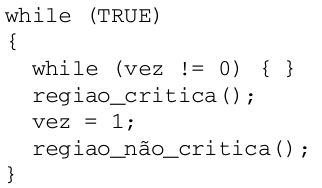
\includegraphics[width=0.9\textwidth]{strict-switch-p1}
    \caption{Código no processo \textbf{\textit{P1}}}
  \end{subfigure}
  ~
  \begin{subfigure}{0.5\textwidth}
    \centering
    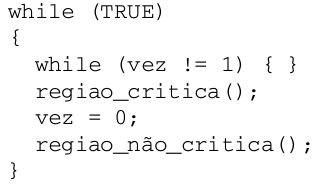
\includegraphics[width=0.9\textwidth]{strict-switch-p2}
    \caption{Código no processo \textbf{\textit{P2}}}
  \end{subfigure}

  \caption{Exemplo clássico de estrita alternância}
  \label{fig:strict-switch}
\end{figure*}

Esta técnica preserva exclusão mútua e a espera limitada. Entretanto, ela \textbf{não preserva o progresso}. Usamos o exemplo da Figura \ref{fig:strict-switch}, dado o caso onde o processo P1 é muito rápido lento que P2. Suponha que P2 está em sua região não-crítica e, nesse meio tempo, P1 executou por inteiro, deixando a variável \texttt{vez} igual a 1. P1 tenta executar o \textit{loop} novamente, mas não irá conseguir até que P2 coloque a variável em 0. Logo, a região crítica está vazia e temos um processo executando fora da região crítica bloqueando um processo que deseja a região.








\subsection{Exclusão Mútua com Bloqueio de Processos}
A outra técnica é o \textbf{bloqueio de processos}, onde o processo que espera a permissão de entrada na seção crítica executa uma primitiva para se bloquear, aguardando até que a seção seja liberada, como na Figura \ref{fig:block-process}.

\begin{figure}[ht]
  \centering
  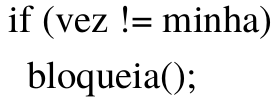
\includegraphics[width=0.35\textwidth]{block-process}
  \caption{Exemplo clássico de bloqueio de processo. O processo checa se as variáveis são iguais e, caso contrário, bloqueia}
  \label{fig:block-process}
\end{figure}

Esta técnica acaba por \textbf{gerar mais trocas de contextos entre processos, causando esperas longas}.

Existem duas primitivas básicas, as quais, normalmente, envolvem a seção crítica:

\begin{itemize}
  \item Primitiva de \textbf{bloqueio de processo} quando a seção estive ocupada;

  \item Primitiva de \textbf{desbloqueio de processos} à espera da permissão de acesso à seção crítica.
\end{itemize}





\subsubsection{Semáforos}
Definidos por \textit{Dijkstra} em 1965, consiste em uma variável inteira positiva, que controla o acesso à região crítica, estabelecendo um limite de controle dos sinais de interesse de acesso à ela. O valor inicial do semáforo indica quantos processos podem acessar o recurso simultaneamente, normalmente inicializado com 1.

As operações de manipulação dos semáforos são \textbf{indivisíveis}, ou seja, se um processo está executando-as, ele não pode ser bloqueado. Elas são duas e seu código é mostrado:

\begin{itemize}
  \item \textbf{\textit{Wait} (P ou \textit{down}):} decrementa o valor do semáforo se este for maior que 0. Caso contrário, o processo que executou a operação é bloqueado;

  \item \textbf{\textit{Signal} (V ou \textit{up}):} incremente o valor do semáforo, acordando qualquer processo que esteja bloqueado.
\end{itemize}

\begin{figure*}[ht]

  \begin{subfigure}[t]{.5\textwidth}
    \centering
    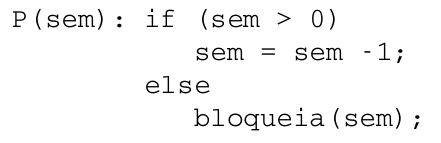
\includegraphics[width=0.9\textwidth]{sem-wait}
    \caption{Operação \textit{Wait}}
    \label{subfig:sem-wait}
  \end{subfigure}
  ~
  \begin{subfigure}[t]{.5\textwidth}
    \centering
    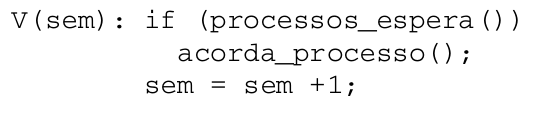
\includegraphics[width=0.9\textwidth]{sem-signal}
    \caption{Operação \textit{Signal}}
    \label{subfig:sem-signal}
  \end{subfigure}

  \caption{Operações de semáforos}
  \label{fig:sem-ops}
\end{figure*}

\textbf{Ideia Geral:} sempre que houver uma região crítica, envolvemos ela com a operação \textit{wait} e \textit{signal}, nesta ordem, como mostra a Figure \ref{fig:semaphore}. Assim, o processo vai checar se o semáforo é maior que 0, ou seja, se a região crítica já está comportando o número limite de processos. Caso esteja, o processo bloqueia, senão, o processo decrementa o valor do semáforo, indicando que há um processo operando ali.
os
Quando o processo acabar de executar a região crítica, ele acorda os outros processos, para que estes possam tentar assumir a região crítica. Finalmente, ele incrementa o semáforo, indicando que há espaço para outro processo acessar o recurso. Note que os outros processos não podem entrar no meio dessas duas ações, pois a ação de \textit{signal} é indivisível.


\begin{figure}[ht]
  \centering
  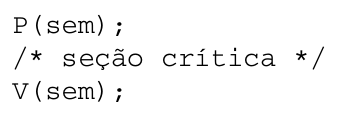
\includegraphics[width=0.35\textwidth]{semaphore}
  \caption{Código de região crítica apropriadamente envolvido por operações de semáforo}
  \label{fig:semaphore}
\end{figure}






\subsubsection{\textit{Locks}}
São estruturas de dados compartilhadas, que garantem a exclusão mútua por \textit{software}, sendo concedido a um processo de cada vez. São operados por duas ações:

\begin{itemize}
  \item \textbf{\textit{Acquire(lock)}:} onde o processo obtém a propriedade do \textit{lock};

  \item \textbf{\textit{Release(lock)}:} onde o processo libera o \textit{lock}.
\end{itemize}

Estas primitivas são chamadas de sistema, podendo ser implementadas tanto como uma espera ocupada ou com bloqueio de processo, sendo este último mais comum e chamado de \textit{mutex}.

\begin{figure}[ht]
  \centering
  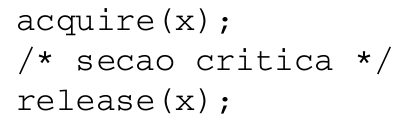
\includegraphics[width=0.35\textwidth]{mutex}
  \caption{Código de região crítica apropriadamente envolvido por operações de \textit{lock}}
  \label{fig:mutex}
\end{figure}


\subsubsection{\textit{Monitores}}
Monitores são conjuntos de procedimentos e dados agrupados em um módulo, indicando que estas entidades são uma região crítica. Estas regiões só podem ser \textbf{acessadas por um processo por vez}, o qual só pode acessar os dados contidos no da seção crítica através de procedimentos definidos pelo monitor. Logo, \textbf{não há acesso direto aos dados por parte do processo requisitante}.

\begin{figure}[ht]
  \centering
  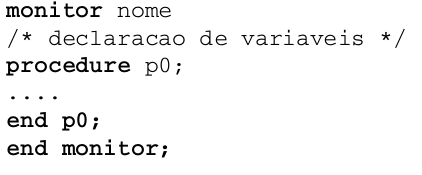
\includegraphics[width=0.55\textwidth]{monitor}
  \caption{Código de região crítica definido dentro de um monitor. Como exemplo, o procedimento \texttt{p0} seria o único com permissão de acessar dados da região crítica}
  \label{fig:monitor}
\end{figure}

O programador é quem definirá as seções críticas, ou seja, o que estará contidos nos monitores. Entretanto, \textbf{a garantia de exclusão mútua é feita pelo compilador}, usando estruturas de baixo nível (como semáforos, por exemplo) e garantindo que apenas um processo acesse o monitor. Por isso, a abstração e \textbf{implementação de monitores deve estar contida na linguagem de programação}, o que raramente é feito.








\subsection{Exemplo Clássico: Produtor-Consumidor}
O problema clássico de Produtor-Consumidor é definido com dois processos \texttt{P0} e \texttt{P1}, que compartilham um \textit{buffer} de tamanho fixo. O processo \texttt{P0} escreve os dados e o processo \texttt{P1} retira-os.

Como o \textit{buffer} tem tamanho fixo, devemos ter uma variável que controle o número de mensagens no mesmo. Assim, o processo produtor não escreve algo quando o \textit{buffer} estiver lotado e o processo consumidor não retira dados quando o \textit{buffer} estiver vazio. Consequentemente, esta variável é compartilhada entre os dois processos, podendo gerar uma condição de corrida.

\begin{figure}[H]
  \centering
  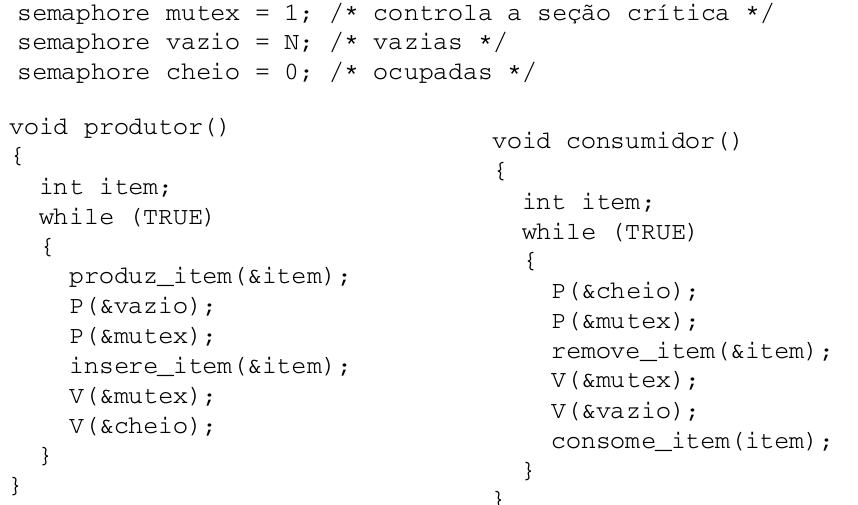
\includegraphics[width=0.75\textwidth]{prod-cons-sem}
  \caption{Solução do problema com semáforos.}
  \label{fig:prod-cons-sem}
\end{figure}

% TODO: colocar o esquema com locks
% \begin{figure}
%   \includegraphics{/path/to/figure}
%   \caption{}
%   \label{}
% \end{figure}

\begin{figure}[H]
  \centering
  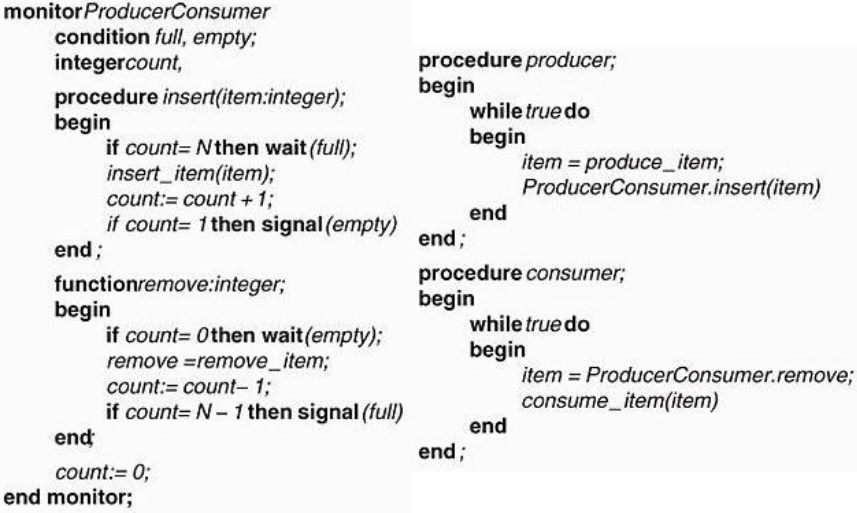
\includegraphics[width=0.85\textwidth]{prod-cons-monitor}
  \caption{Solução do problema com monitores. Definida a variável crítica \texttt{count}, apenas os procedimentos \texttt{insert} e \texttt{remove} podem opera-la. A lógica dos processos são realocadas em procedimentos distintos}
  \label{fig:prod-cons-monitor}
\end{figure}









\section{Troca de Mensagens entre Processos}
Em \textbf{ambientes distribuídos}, onde não há uma memória física compartilhada, as técnicas de compartilhamento de variável acabam por serem ineficazes. Logo, gerou-se a necessidade da troca de mensagens entre os processos para haver a comunicação entre estes. Note que este método pode ser implementado também em ambientes de memória física compartilhada.

A troca de mensagem entre processos é explicita, onde toda comunicação existe no ato de um processo enviar a mensagem e o outro receber. O momento onde a troca ocorre de fato é chamado de \textbf{rendez-vous}. Portanto, há apenas duas primitivas: enviar a mensagem (\textit{send}) e recebê-la (\textit{receive}).

Quando projetamos a comunicação, devemos nos preocupar com alguns aspectos das primitivas. Por exemplo, a cardinalidade: 1 para 1, 1 para $n$ ou $n$ para $n$. Também é importante se preocupar se as primitivas devem ser bloqueadas ou não, ou seja, antes de concluir o \textit{rendez-vouz}, se o processo remetente deve ser bloqueado ou não.

\begin{figure}[h]
  \centering
  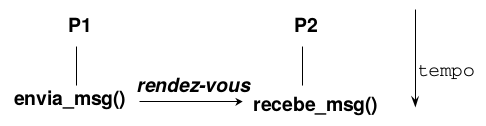
\includegraphics[width=0.7\textwidth]{message-exchange}
  \caption{Ilustração de um \textit{rendez-vouz}}
  \label{fig:rendez-vouz}
\end{figure}

É importante ressaltar que a maioria dos sistemas \textbf{permitem ambas as abordagens de comunicação}, inclusive permitindo o programador misturar primitivas das duas.

\subsection{Primitivas Bloqueadas}
Primitivas bloqueadas ocorrem quando, em um envio de mensagem, o processo remetente é bloqueado até que o \textit{rendez-vouz} aconteça, ou seja, até que o processo destinatário execute a primitiva de recebimento.

Podemos ter dois comportamentos:
\begin{itemize}
  \item \textbf{\textit{Send} antes do \textit{Receive}:} primeiro, o processo remetente envia a mensagem e se bloqueia, aguardando o \textit{rendez-vouz}. O processo destinatário se bloqueia apenas para receber a mensagem, desbloqueando logo depois. \textbf{O maior tempo de bloqueio está do lado do remetente};

  \item \textbf{\textit{Receive} antes do \textit{Send}:} primeiro, o processo destinatário se bloqueia, aguardando a mensagem, desbloqueando apenas quando recebe. O processo remetente se bloqueia apenas no momento do envio da mensagem e logo recomeça a execução. \textbf{O maior tempo de bloqueio está do lado do destinatário}.
\end{itemize}

\begin{figure*}[ht]
  \begin{subfigure}[t]{0.5\textwidth}
    \centering
    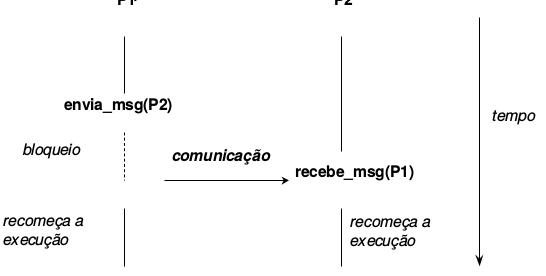
\includegraphics[width=0.85\textwidth]{block-send-receive}
    \caption{\textit{Send} antes do \textit{receive}}
    \label{subfig:block-send-receive}
  \end{subfigure}
  ~
  \begin{subfigure}[t]{0.5\textwidth}
    \centering
    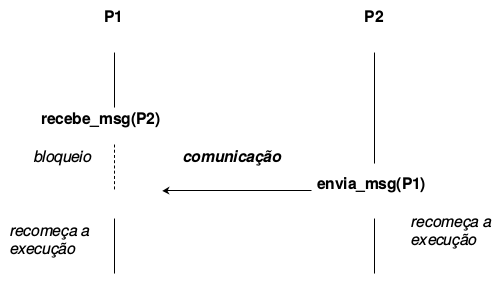
\includegraphics[width=0.85\textwidth]{block-receive-send}
    \caption{\textit{Receive} antes do \textit{send}}
    \label{subfig:block-receive-send}
  \end{subfigure}

  \caption{Tipos de comportamento para primitivas blocantes}
  \label{fig:blocking-types}
\end{figure*}

Dizemos que essa é uma \textbf{comunicação síncrona}, dado que no memento da troca de mensagens, cada processo envolvido na comunicação sabe exatamente o estado do outro, pois ambos estão executando a primitiva de comunicação. Logo, implicitamente os processos também estão comunicando os seus estados de execução. Como vantagem, estas primitivas \textbf{tem implementação mais simples}.

Quando dois processos executam um \textit{receive}, esperando um mensagem do outro, ambos se encontram bloqueados e aguardando um recurso do outro. Logo, vemos a \textbf{possibilidade de \textit{deadlock}} nesta comunicação. Tal situação pode ser resolvida com a temporização da primitiva de \textit{receive}, estabelecendo um tempo máximo que o processo pode ficar bloqueado.

\begin{figure*}[ht]
  \begin{subfigure}[t]{0.5\textwidth}
    \centering
    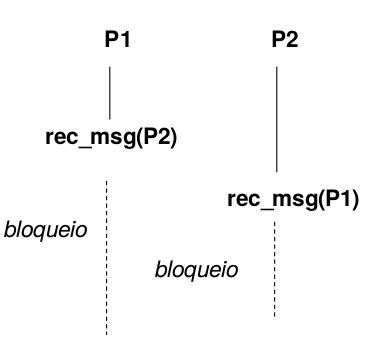
\includegraphics[width=0.7\textwidth]{block-deadlock}
    \caption{Possível \textit{deadlock}}
    \label{subfig:block-deadlock}
  \end{subfigure}
  ~
  \begin{subfigure}[t]{0.5\textwidth}
    \centering
    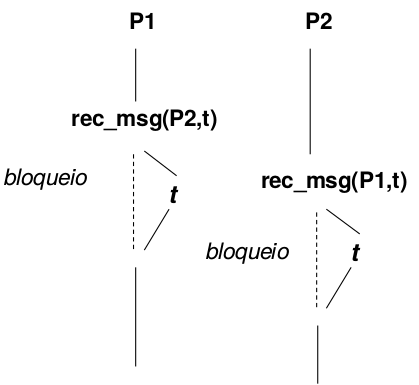
\includegraphics[width=0.7\textwidth]{block-temporizer}
    \caption{Solução com temporizadores}
    \label{subfig:block-temporizer}
  \end{subfigure}

  \caption{Possível desvantagem ao utilizar primitivas blocantes}
  \label{fig:block-deadlock-scheme}
\end{figure*}

Outra desvantagem é a \textbf{perda de paralelismo}, causada pela primitiva blocante. Um contorno para este problema é a utilização de \textit{threads} para realizar as primitivas, o que é chamado de \textbf{comunicação pseudo-assíncrona}. Tal abordagem está sendo muito estudada por juntar o melhor dos mundos das abordagens síncronas e assíncronas.

\begin{figure*}[ht]
  \begin{subfigure}[t]{0.5\textwidth}
    \centering
    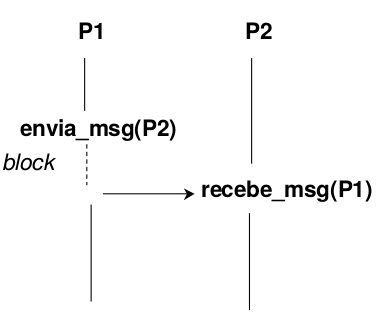
\includegraphics[width=0.7\textwidth]{block-blocking}
    \caption{Problema de perda de paralelismo}
    \label{subfig:block-pseudo-async1}
  \end{subfigure}
  ~
  \begin{subfigure}[t]{0.5\textwidth}
    \centering
    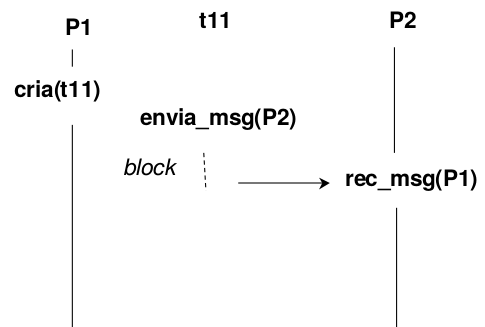
\includegraphics[width=0.7\textwidth]{block-pseudo-async}
    \caption{Solução com \textit{thread}}
    \label{subfig:block-pseudo-async2}
  \end{subfigure}

  \caption{Problema e solução com primitivas pseudo-assíncronas}
  \label{fig:block-pseudo-async}
\end{figure*}


\subsection{Primitivas Não-Bloqueadas}
Aqui, tanto o processo remetente como o destinatário não são bloqueados ao realizar as primitivas. Logo, esta técnica \textbf{oferece um alto grau de concorrência}.

Assim como nas síncronas, temos dois comportamentos. Quando o \textit{send} vem antes do \textit{receive}, o remetente simplesmente envia a mensagem, sem bloquear, e o remetente recebe a mesma, ambos usando as primitivas padrões.

\begin{figure}[ht]
  \centering
  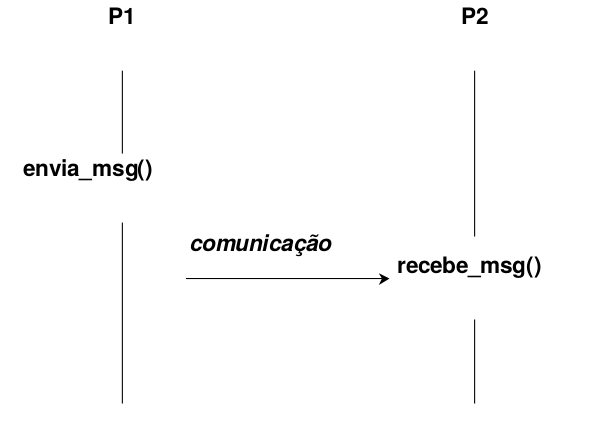
\includegraphics[width=0.5\textwidth]{nonblock-sendreceive}
  \caption{\textit{Send} antes de \textit{receive} em primitivas não-blocantes}
  \label{fig:nonblock-sendreceive}
\end{figure}

Entretanto, como o \textit{receive} não é blocante, na estratégia de \textit{receive} antes do \textit{send} é capaz que a mensagem esperada do remetente ainda não tenha chegado. Para isso, existem duas abordagens:

\begin{itemize}
  \item \textbf{NOMSG:} ao constatar o não recebimento da mensagem, a primitiva retorna um sinal de \textit{mensagem não recebida} (\texttt{NOMSG}) para o processo;

  \item \textbf{\textit{Probing}:} ao constatar o não recebimento da mensagem, é feita uma primitiva que requisita a mensagem ao remetente. Em certas situações, essa primitiva pode acarretar no bloqueio do destinatário (note que ela não é um \textit{send} ou \textit{receive}).
\end{itemize}

\begin{figure*}[ht]
  \begin{subfigure}{0.5\textwidth}
    \centering
    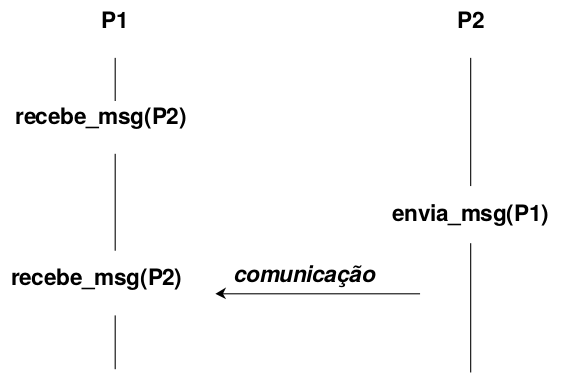
\includegraphics[width=0.7\textwidth]{nonblock-nomsg}
    \caption{Abordagem com \texttt{NOMSG}}
    \label{subfig:nonblock-nomsg}
  \end{subfigure}
  ~
  \begin{subfigure}{0.5\textwidth}
    \centering
    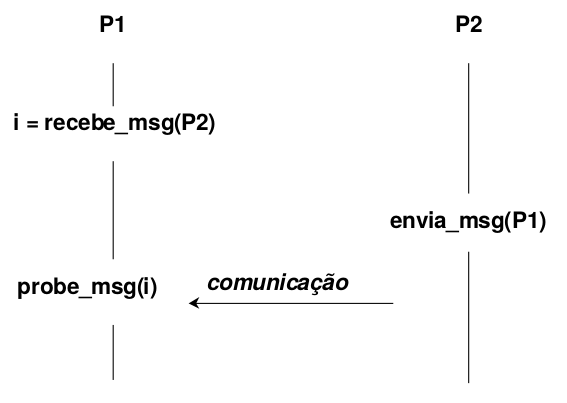
\includegraphics[width=0.7\textwidth]{nonblock-probing}
    \caption{Abordagem com \textit{probing}}
    \label{subfig:nonblock-probing}
  \end{subfigure}

  \caption{Comportamentos para \textit{receive} antes de \textit{send} em primitivas não-blocantes}
  \label{fig:messages-nonblock}
\end{figure*}

	\chapter{Memória}
De uma maneira geral, quando um processo é criado, sua imagem (ou parte dela) é armazenada em memória, onde a as instruções e os dados que estão sendo manipulados em um determinado instante são carregados na CPU. Os dados alterados são escritos em memória continuamente e os mais permanentes são armazenados em disco.

Um programa fonte apresenta instruções contendo endereços simbólicos, definidos pelo programador. Após o processo de compilação e montagem, o programa agora apresenta endereços relocáveis, construído em relação ao início do módulo objeto. Após a \textit{linkagem}, o programa agora possui os endereços absolutos, únicos para o programa como um todo.

















\section{Gerenciamento}
O gerenciamento de memória é implementado pelo \textbf{gerente de memória}, responsável por definir e implementar a política de gerenciamento de memória do SO. Além disso, independente desta política, o gerente deve controlar a alocação das porções de memória aos processos, liberando-as quando estas não forem mais necessárias. As técnicas de gerênciamento são três: \textit{monitor residente}, \textit{multiprogramação} e \textit{memória virtual}.






\subsection{Monitor Residente}
Em sistemas monoprogramados, a memória é geralmente dividida em duas áreas: uma para o usuário e outra para o sistema operacional.

Dessa forma, apenas um processo usuário está ativo por vez, pois a área de usuário é destinada a um processo apenas. Da mesma forma, a área do SO é ocupada por ele, o qual está sempre ativo.

Entretanto, é necessário um \textit{hardware} adicional, o qual vai impedir que processos de usuário invadão a área de memória do SO. É instaurada uma barreira, delimitando as áreas de memória, e a todo cálculo de endereço do processo usuário, o resultado é checado. A Figura \ref{fig:memory-fence} resume o processo.

\begin{figure}
  \centering
  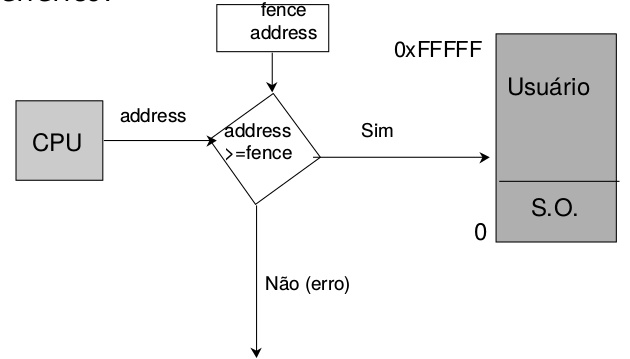
\includegraphics[width=0.65\textwidth]{memory-fence}
  \caption{O processo na CPU tentar acessar um endereço da memória. O \textit{hardware} checa se este endereço respeita o limite de área de memória do SO, liberando o acesso em caso positivo ou lançando um erro em caso negativo}
  \label{fig:memory-fence}
\end{figure}

Como \textbf{vantagens}, esta técnica tem implementação simples, pois só há um pequeno componente de proteção sendo usado. Além disso, os serviços do sistema operacional podem ser utilizados, como \textit{drivers}, interrupções, etc..

Como \textbf{desvantagem}, temos uma CPU sub-aproveitada, onde o sistema pode ser apenas mono-usuário e mono-tarefa






\subsection{Multiprogramação}
Multiprogramação é ofertada pela maioria dos computadores, onde vários processos coexistem na memória, havendo a necessidade da proteção de suas respectivas áreas de memória, evitando que um processo acesse a área de outro.

Logo, é lançado mão dos \textbf{registradores de base e limite}, definido dois limites de memória para o processo. Durante a execução, cada endereço usado para acessar a memória é adicionado ao valor contido no registrador de base, afim de obter o endereço físico onde o dado reside. Este registrador implementa a relocação.

Caso o endereço ultrapasse o valor do registrador limite, um erro é emitido. Assim, este registrador implementa a proteção de memória.







\subsection{Memória Virtual}
A memória virtual surgiu como uma solução para o problema de se alocar espaço em memória para um processo que não cabe inteiramente nela. Ou seja, temos um \textbf{processo com tamanho maior que o da memória física}.

A solução é quebrar o processo em unidades menores, carregando-as a medida que elas são necessárias. O problema é quem vai quebrar o processo: o programador ou o sistema operacional? Caso for o primeiro, temos um \textit{overlay} e do segundo, nasceu a memória virtual.

Proposto em 1961, é o método mais comum atualmente, considerando os SO atuais, sendo um mecanismo genérico sendo suportado tanto por sistemas mono e multiprogramados. Logo, a idéia é referenciar mais endereços virtuais e não endereços físicos. Logo, parte do SO a responsabilidade de definir os módulos de memória e suas alocações.

\textbf{O número de endereços virtuais depende da capacidade de endereçamento da máquina} e do suporte do SO. Na execução de cada instrução, os endereços virtuais devem ser traduzidos para endereços físicos, o que exige um cálculo. Temos dois modelos para implementação da memória virtual:

\begin{itemize}
  \item \textbf{Paginação:} divide a memória física e a memória virtual em unidades de \textbf{tamanho fixo};

  \item \textbf{Segmentação:} divide a memória física e a memória virtual em unidades de \textbf{tamanho variável}.
\end{itemize}

Para ilustrar o possível espectro de endereços virtuais, supomos um arquitetura de 32 \textit{bits}. Logo, um processo pode endereçar até $2^{32} - 1$ endereços, independente da memória física.





\section{Espaço de Memória}

\subsection{Swapping}
\begin{definicao}{\textit{Swapping}}
  Movimento de processos \textbf{ativos} da memória para o disco e vice-e-versa.
\end{definicao}

Geralmente, a memória disponível no computador não é capaz de armazenar todos os processos ativos em um dado instante. Como não há espaço físico na memória, devemos colocar alguns processos ativos em disco. Normalmente, existe uma área em disco reservada para tal, chamada de \textbf{área de \textit{swap}}.

Definimos o movimento de memória para o disco como \textit{swap-out}. O movimento de disco para memória é o \textit{swap-in}.



\subsection{Alocação de Espaço}
O problema da alocação de espaço para processos é o problema de determinar a quantidade de memória que devemos reservar para um processo. Em sistemas onde um processo tem tamanho fixo, alocamos uma quantidade de memória exatamente igual ao tamanho do código binário do processo.

Infelizmente, a maioria dos sistemas permite que o tamanho da área de dados de um processo cresça ao longo da execução. Neste caso, é interessante alocar um espaço de memória maior que o tamanho inicial do processo, de forma a evitar o movimento do mesmo no caso de crescimento da sua área de dados.

Para tal, temos duas maneiras de implementar este controle: \textit{mapa de bits} e \textit{lista encadeada}.


\subsubsection{Mapa de \textit{Bits}}
Aqui a memória é dividida em unidade de alocação (\textit{UAs}) de tamanho fixo, onde cada uma corresponde a um \textit{bit} no mapa. Se a unidade estiver livre, o valor é 0, caso contrário, o valor é 1.

\begin{figure}[h]
  \centering
  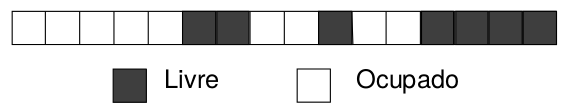
\includegraphics[width=0.5\textwidth]{memory-bitmap}
  \caption{Mapa de \textit{bits} associado à memória, com cadeia 1111100110110000}
  \label{fig:memory-bitmap}
\end{figure}


\subsubsection{Lista Encadeada}
Aqui as cadeias de segmentos livres e ocupados são representados através de um lista encadeada, onde cada entrada contém o tipo do segmento (livre ou ocupado), o endereço de início e um ponteiro para o próximo elemento. Desta forma, o percorrimento e busca por espaços é mais rápido.

Existem variações que implementam listas duplamente encadeadas, para que seja possível fazer o \textit{merge} de buracos. Tal situação é comum quando ocorre um término de processo.

\begin{figure}[h]
  \centering
  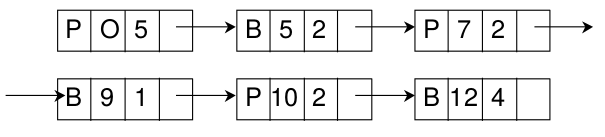
\includegraphics[width=0.6\textwidth]{memory-chained-list}
  \caption{Representação de lista encadeada para o contexto de memória da Figura \ref{fig:memory-bitmap}}
  \label{fig:memory-chained-list}
\end{figure}
















\section{Paginação}
Paginação é uma técnica de memória virtual, onde é utilizado um endereço virtual que representa um \textbf{espaço de endereçamento virtual} dividido em unidades de tamanho fixo, chamadas de \textbf{páginas}, e a memória física é dividida em unidades de tamanho fixo chamadas \textbf{\textit{page frames}}. Estas últimas, serão as áreas de memória física que irão abrigar as páginas utilizadas pela CPU.

A tradução entre páginas e \textit{frames} tem auxílio de um \textit{hardware} adicional, chamado \textbf{Memory Management Unit (MMU)}, o qual recebe um endereço virtual, mapeando-o no seu endereço físico correspondente, e escreve este último no barramento da memória, a qual poderá retornar o dado desejado para a CPU. A indexação de endereços é feita por uma estrutura interna da MMU chamada \textbf{tabela de páginas}.

\textbf{Nota:} se estas operações fossem feitas por \textit{software}, o esquema de paginação sera comprometido pelo alto \textit{overhead} a cada acesso.

\begin{figure}[h]
  \centering
  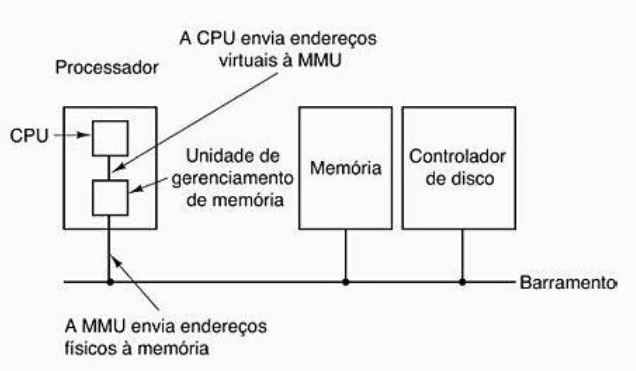
\includegraphics[width=0.75\textwidth]{pagination-overview}
  \caption{Esquema geral da paginação}
  \label{fig:pagination}
\end{figure}










\subsection{\textit{Page Fault}}
O espaço de endereçamento virtual é geralmente bem maior que o espaço de memória física. Dessa forma, é comum que uma página solicitada da CPU não esteja mapeada em memória física.

Por isso, a MMU possui em sua estrutura o \textit{bit} de presença, que indica a presença ou não da página na memória. Caso o \textit{bit} indique que não, a MMU irá \textbf{emitir uma \textit{trap} para o SO, chamado de \textit{page fault}}.

Dessa forma, o SO irá escolher uma página da memória para ser substituída pela página requisitada. A página requisitada é buscada em disco e inserida na memória, enquanto a página substituída é retirada da memória e inserida em disco. Por fim, a tabela de páginas é devidamente alterada, com a troca do \textit{bit} de presença e a instrução que gerou a requisição da memória é reexecutada. a Figura \ref{fig:page-fault} ilustra o processo.

\begin{figure}
  \centering
  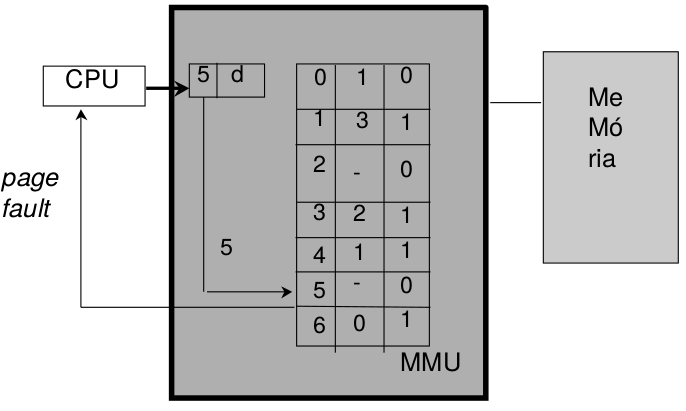
\includegraphics[width=0.7\textwidth]{page-fault}
  \caption{Esquema geral de um \textit{page fault}}
  \label{fig:page-fault}
\end{figure}











\subsection{Tabela de Páginas}
\begin{definicao}{Tabela de Páginas}
  Estrutura de dados presente na MMU que guarda as informações necessárias para o mapeamento do endereço virtual de um processo em endereços físicos.
\end{definicao}

As tabelas de página podem variar entre máquinas diferentes, porém possuem campos comuns:
\begin{itemize}
  \item \textbf{\textit{Bit} de \textit{cache}}: indica se a página pode ser colocada em \textit{cache};

  \item \textbf{\textit{Bit} de referência:} indica se a página foi referenciada;

  \item \textbf{\textit{Bit} de modificação:} indica se a página foi alterada;

  \item \textbf{\textit{Bit} de proteção:} indica a proteção associada à página;

  \item \textbf{\textit{Bit} de presença:} indica se a página está mapeada em memória física;

  \item \textbf{Número do \textit{frame}:} número do \textit{frame} onde a página está mapeada.
\end{itemize}

Observe que \textbf{o tamanho da tabela de páginas depende do espaço de endereçamento da arquitetura}. Dessa forma, a tabela poderia assumir espaços irreais como $2^{64}$. Dessa forma, dois problemas são inseridos: não é viável manter a tabela totalmente na MMU e a velocidade de mapeamento dos endereços pode ser comprometida.

Para mitigar o problema do tamanho, a \textbf{tabela de páginas fica armazenada em memória principal}, onde um registrador guarda o endereço de início desta tabela. Logo, a MMU utiliza uma memória associativa chamada de \textbf{\textit{Translation Look-aside Buffer} (TLB)}, onde algumas entradas da tabela de páginas são armazenadas.

Assim, quando um endereço virtual é apresentado a MMU, ela procura este na TLB. Se estiver presente, o mapeamento é direto, caso contrário, um acesso à memória é feito para recuperar a entrada da tabela de páginas. A entrada requisitada é inserida na TBL, de forma que futuras requisiçõe serão imediatas.

Temos duas organizações possíveis para a tabela de páginas: mapeamento direto ou invertida.

\subsubsection{Mapeamento Direto}
Também chamada de \textit{forward-mapped}, aqui a \textbf{tabela de páginas é um vetor de entradas armazenadas em memória}. Existe uma entrada para cada página e a \textit{frame} é obtida a partir desta.

Para este esquema \textbf{cada processo tem uma tabela de páginas}. Aliado ao crescimento do espaço de endereçamento e tamanho da página, as tabelas acabam por ficarem grandes demais. Dessa forma, para evitar que essas tabelas fiquem em memória o tempo todo, os computadores implementam as \textbf{tabelas de página em  multinível}.

Esta organização faz com que mesmo que um processo possa armazenar $2^n$ posições em memória física, ele não vai fazer isto. Logo, o número da página é quebrado em $n$ partes, onde $n$ será o número de níveis. A Figura \ref{fig:forward-mapped} ilustra a divisão.

\begin{figure}[h]
  \centering
  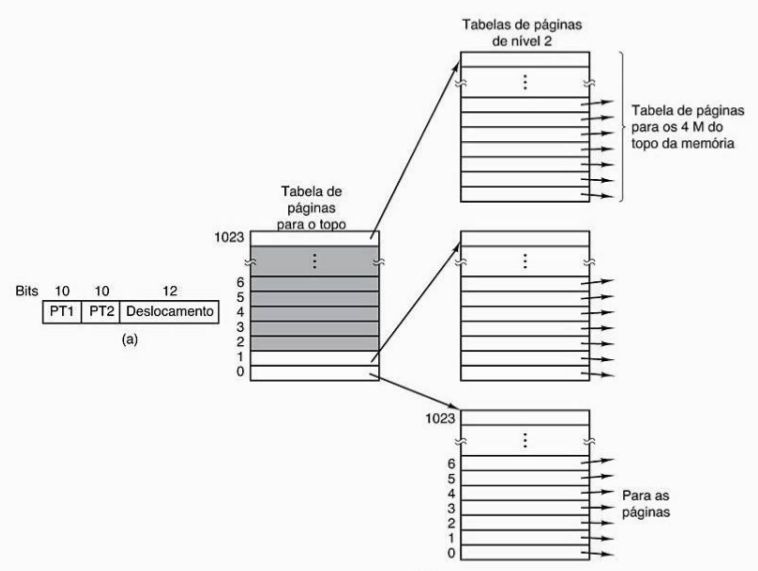
\includegraphics[width=0.8\textwidth]{forward-mapped}
  \caption{Tabelas de página de dois níveis, para um enderaçmento de 32 \textit{bits}}
  \label{fig:forward-mapped}
\end{figure}

Como exemplo, existem tabelas de páginas de 1 nível (PDP-11), 2 níveis (VAX), 3 níveis (SunSPARC) e 4 níveis (Motorola 68030). Além de 4 níveis, o projeto fica extremamente complexo e o ganho não é muito grande.




\subsubsection{Mapeamento Invertido}
Com processadores em 64 \textit{bits} e páginas com $4KB$, acabamos por ter $2^{52}$ entradas na tabela de página, o que torna inviável a utilização de tabelas com mapeamento direto. \textbf{Nota:} mesmo assim. algumas arquiteturas de 64 \textit{bits} utilizam este mapeamento, com 3 níveis.

Em tabelas de páginas invertidas, a indexação é feita pelo \textit{frame} e não mais pela página. O problema é que o índice utilizado pela CPU ainda é a página $p$. Por isso, neste método é utilizada uma tabela de \textit{hash}, com o \textit{frame} como índice. Logo, a CPU envia $p$ como entrada, porém antes de ser aplicado na tabela, é feito um \textit{hash} sobre $p$ para obter o índice correspondente. \textbf{Nota:} em particular, esse \textit{hash} é uma função de módulo, dado que o tamanho da tabela é o tamanho de \textit{frames} possíveis na memória.

Entretanto, existem páginas que após o \textit{hash} acabam por cair no mesmo índice. Nelas, são criados \textit{buckets} (lista de conflitos) contendo o endereço da página virtual $p$ e o \textit{frame} $f$ correspondente a ser escrito no barramento.












\subsection{Substituição de Páginas}
A condição de um bom algoritmo de substituição é de escolher sempre a página a página que está em memória física que será referenciada no futuro mais distante. Entretanto, isso não é possível pois não há como saber o futuro. Portanto, usamos estratégias realizáveis.

\subsubsection{NRU}
Abreviação de \textit{Não recentemente utilizada}, este método utiliza os \textit{bits} de referência ($R$) e de modificação ($M$). contidos na tabela de página.

O \textit{bit} $R$ sempre é setado para 1 quando a página associada for acessada, tanto para leitura como escrita. O \textit{bit} $M$ é setado para 1 sempre que a página for modificada, ou seja, apenas escrita. Todas estas atualizações são feitas em \textit{hardware}.

Quando o contexto do processo é carregado, os dois \textit{bits} são zerados e periodicamente, o SO zera o \textit{bit} R. Logo, quando há um \textit{page fault}, o SO analisa as páginas e as categoriza da seguinte forma:

\begin{itemize}
  \item \textbf{Classe 0:} não referenciada, não modificada ($R = 0 \mid M = 0$);

  \item \textbf{Classe 1:} não referenciada, modificada ($R = 0 \mid M = 1$);

  \item \textbf{Classe 2:} referenciada, não modificada ($R = 1 \mid M = 0$);

  \item \textbf{Classe 3:} referenciada, modificada ($R = 1 \mid M = 1$);
\end{itemize}

Dessa forma, o SO escolhe a página não-vazia da classe mais baixa e a substitui.

\textbf{Nota:} observe que para ter uma página não referenciada, mas modificada, é preciso que o SO tenha zerado o \textit{bit} de referência, o que ele faz periodicamente.



\subsubsection{FIFO}
Abreviação de \textit{first in, first out}, o FIFO usa a política de substituição da página que foi carregada a mais tempo. As páginas em memória são mantidas em uma fila organizada por idade. A página mais antiga no início e mais recente no final.

Quando ocorre o \textit{page fault}, a página removida é aquela que está no início da fila e a página que causou o \textit{page fault} é colocada no final.

Apesar de ser um algoritmo simples de se implementar, nada garante que uma página carregada a muito tempo não seja mais utilizada, dado que a utilização da página não está relacionada com o seu tempo de carga. Por isso, este algoritmo é raramente utilizado.




\subsubsection{Segunda Chance}
Este algoritmo é uma modificação do FIFO. Quando há um \textit{page fault}, o algoritmo analisa a página carregada há mais tempo. Se o seu \textit{bit} $R$ for 0, a página é escolhida para substituição. Entretanto, se $R$ for 1, o mesmo é zerado e a página colocada no final da fila, ou seja como mais recente. A busca continua até que haja uma página onde $R$ seja 0 e esta é escolhida.

Dessa forma, vemos que o algoritmo procura uma página que tenha sido carregada a muito tempo e não tenha sido referenciada. Se todas as páginas tiverem sido referenciadas, ele degenera para um FIFO.


\subsubsection{Relógio}
Utiliza a mesma filosofia do algoritmo de segunda chance, porém não utiliza filas simples para armazenar as páginas. As páginas são mantidas em uma fila circular, com um ponteiro que aponta para a página mais antiga.

Quando há um \textit{page fault}, o algoritmo analisa a página apontada pelo ponteiro. Se o seu \textit{bit} $R$ for 0, a página é escolhida para substituição. Caso seja 1, o \textit{bit} é zerado e o ponteiro aponta para a próxima página. A busca continua até que haja uma página onde R seja 0. A diferença está na substituição: a página inserida não é posta no fim de uma fila, mas assume a posição da página retirada.



\subsubsection{LRU}
Dado o princípio da localidade, páginas muito referenciadas nas últimas instruções tem grande chance de serem referenciadas pelas instruções futuras. Da mesma maneira, páginas não referenciadas há muito tempo tem grande probabilidade de continuarem a não serem utilizadas por muito tempo.

Portanto, o \textit{Least Recently Used} (LRU) se aproveita deste princípio e tenta escolher a página que foi referenciada no passado mais distante para ser substituída.

Teoricamente, ele tem bons resultados, mas sua implementação é custosa, dado que é necessário implementar uma lista encadeada organizada pelo tempo de último acesso. Dado isso, algumas técnicas de implementação do LRU acabam utilizando um \textit{hardware} especial. Entretanto, para SOs genéricos, o mais comum é a simulação de \textit{software} do LRU, que é chamada de \textit{Não Frequentemente Utilizada}, ou NFU.

No NFU necessitamos de um contador adicional, a ser mantido em tabela de páginas, para página. Periodicamente, o SO percorre todas as páginas em memória, adicionando o valor do \textit{bit} R de cada página ao seu contador. Quando ocorre um \textit{page fault}, página escolhida é aquela que possui o menor contador.

O problema do NFU é que uma página muito referenciada há muito tempo atrás raramente é escolhida para substituição, pois o NFU não "esquece" tais referencias passadas.


\subsubsection{NFU com \textit{Aging}}
Para que as referência antigas do NFU sejam esquecidas, devemos utilizar uma técnica chamada \textit{aging}. O número de \textit{bits} no contado é o número de referências passadas que será considerado.

No \textit{aging}, a cada interrupção de \textit{clock}, é feito um \textit{shift} do contador de cada página para a direita e o \textit{bit} R é inserido à esquerda, ou seja, no \textit{bit} mais significativo. Quando há um \textit{page fault}, o algoritmo escolhe a página com o menor contador. A Figura \ref{fig:nfu-aging} mostra o funcionamento.

\begin{figure}[h]
  \centering
  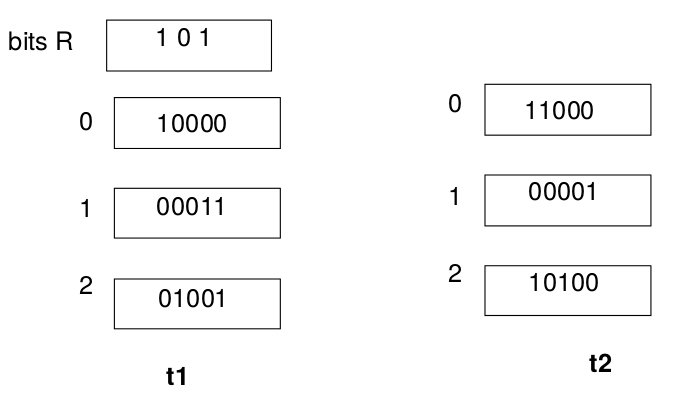
\includegraphics[width=0.7\textwidth]{nfu-aging}
  \caption{\textit{Shift} do NFU em dois tempos distintos adjacentes}
  \label{fig:nfu-aging}
\end{figure}




\subsection{Tratamento de \textit{Page Fault}}
Aqui é explicada toda a rotina de tratamento de um \textit{page fault}:

\begin{enumerate}
  \item O \textit{hardware} gera um \textit{trap} para o \textit{kernel} e salva o PC corrente na pilha;

  \item O \textit{hardware} executa uma rotina em código de máquina, que salva os demais registradores e outras informações. No final, a rotina chama o SO;

  \item O SO recebe o \textit{trap} e determina que ocorreu um \textit{page fault}. O mesmo determina a página virtual necessária para a resolução do \textit{page fault}, o qual geralmente está em um registrador especial;

  \item Com o endereço virtual em falta, o SO verifica se o endereço é válida e se houve a violação de proteção;

  \item O SO determina um espaço de \textit{frame} livre para inserir a página solicitada. Caso não haja, o algoritmo de subtituição é executado. Se a página selecionada tiver sido modificada, ela deve ser escrita em disco. O \textit{frame} é marcado como reservado e o SO escolhe um novo processo para rodar;

  \item Quando o SO tem certeza de que o \textit{frame} está livre, ele determina o endereço de disco onde se encontra a página que causou o \textit{page fault}. Durante a busca no disco para a passagem para a memória, um novo processo é posto para rodar;

  \item Ao checar a interrupção de disco que indica o términa da cópia da página de disco para memória, a tabela de páginas é alterada e o \textit{frame} é marcado como ocupado;

  \item A instrução que causou o \textit{page fault} é carregada no registrador de instruções e o seu endereço é carregado no PC. Daí, o processo desta instrução é colocado para rodar. O SO termina a execução, voltando a ser executada a rotina em código de máquina que o chamou. A rotina restaura os registradores e demais informações para a situação anterior à falta e dá o processador ao processo de usuário;

\end{enumerate}








\subsection{Funcionamento Detalhado}
Aqui descrevemos o funcionamento geral do pedido de uma página pela CPU. Supondo um processo na CPU que requisite um dado da memória:

\begin{enumerate}
  \item A CPU envia o endereço virtual $v$ à MMU;

  \item Na MMU, o endereço virtual é divido em uma tupla ($p,d$), onde $p$ é a página desejada e $d$ o deslocamento dentro da página;

  \item Ainda na MMU, a página $p$ é utilizada para acessar a \textbf{tabela de páginas}, que reside na MMU. A partir dessa tabela, a tupla inicial é convertida na tupla $F = (F,d)$ correspondente do endereço físico. Nela, $f$ corresponderá ao \textit{frame} da memória física e o deslocamento permanece o mesmo;

  \item Antes de escrever o endereço no barramento, a MMU checa se a página está mapeada em memória física, através de um \textit{bit} de presença.

  \begin{itemize}
    \item Caso a página esteja mapeada, o endereço já pode ser escrito no barramento;

    \item Caso contrário, a MMU gerá um \textit{syscall} ao SO, chamado de \textbf{\textit{page fault}}. Dessa forma, seleciona um \textit{frame} da memória pra ser substituído pela página requisitada e a instrução inicial de acesso a memória é reexecutada. Consequentemente, a MMU vai constatar que a página existe;
  \end{itemize}

  \item O endereço físico $F$ é escrito no barramento de memória
\end{enumerate}


\subsubsection{Cálculos na Paginação}
Em uma arquitetura com espaço de endereçamento de $b$ \textit{bits}, páginas de tamanho $P$ \textit{bytes} e uma memória RAM com tamanho $M$ \textit{bytes}, temos que:

\begin{itemize}
  \item O número de endereços virtuais possíveis é de $2^b$;

  \item O número $F$, que é o total de \textit{frames} na RAM é dado por:

  \begin{equation*}
    F = \frac{M}{P}
  \end{equation*}
\end{itemize}

Ao solicitar um endereço virtual à memória, a CPU utiliza a tupla $(p,d)$, onde $p$ é a página virtual e $d$ o deslocamento dentro da página. Este endereço virtual deve ser transformado em um endereço físico \textbf{de mesmo tamanho}, composto pela tupla $(f,d)$, onde $f$ é o número do \textit{frame} a ser utilizado e $d$ é o mesmo deslocamento usado no endereço virtual.

Disso, temos que:

\begin{itemize}
  \item O tamanho de página $P$ é o valor máximo que $2^d$ pode assumir;
\end{itemize}

	\chapter{Entrada e Saída}

Para prover um abstração simples da máquina física, o sistema operacional deve conhecer bem cada \textit{hardware} sobre o qual ele opera, uma vez que cada um destes dispositivos tem um conjunto de comandos específicos. As unidades de entrada e saída são compostas por duas partes: uma parte mecânica, sendo o dispositivo propriamente dito, e uma parte eletrônica, que é a sua \textbf{controladora}, a qual irá interagir com o SO para realizar as operações de E/S.

\begin{figure}[H]
  \centering
  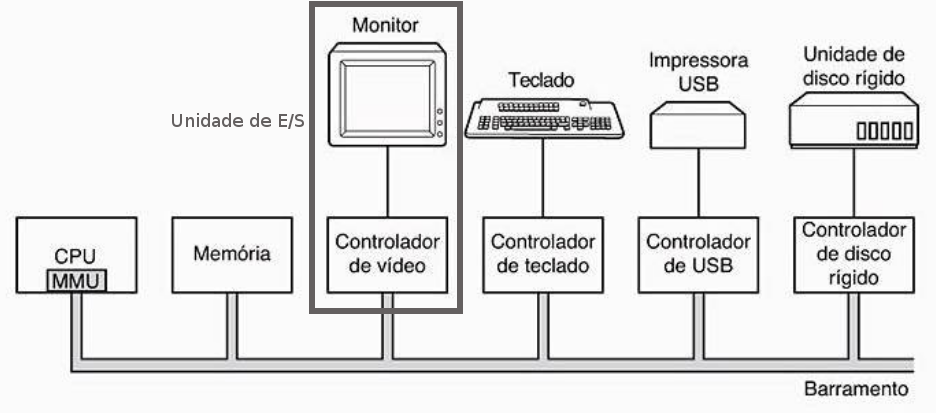
\includegraphics[width=.8\textwidth]{io-unity}
  \caption{Diversas unidades de entrada e saída do SO. Os dispositivos mecânicos estão ligados às suas respectivas controladoras.}
  \label{fig:io-unity}
\end{figure}

A \textbf{comunicação entre SO e controladora} se dá por registradores acessados pela CPU, onde o SO emite comandos escrevendo nestes e obtém informações sobre os dispositivos por meio da leitura dos registradores. Além disso, parte da comunicação também é feita por \textit{buffers}, onde o SO lê e escreve dados. Cada controladora irá possuir um conjunto de comandos específicos, definidos em seus manuais.

Os registradores de controle podem estar localizados nas controladores, sendo mapeados em portas de E/S. Entretanto, o sistema geralmente empregado é o de \textbf{E/S mapeado em memória}, onde os registradores são mapeados em posições fixas da memória, sendo associado um endereço a eles.

Em um processo genérico de E/S, temos que:
\begin{enumerate}
  \item A CPU envia um sinal ao barramento, contendo o endereço desejado, a operação (\textit{read}/\textit{write}) e espaço do registrador (controladora/memória);

  \item O dispositivo referênciado responde a requisição, emitindo uma chamada de sistema ao fim do serviço.
\end{enumerate}

Por fim, em geral, dividem-se os dispositivos de entrada e saída em dois tipos:
\begin{itemize}
  \item \textbf{Dispositivos de Bloco:} onde temos informações sendo armazenadas em unidades de tamanho fixo e sua recuperação é feita por acesso direto. \underline{Exemplo:} disco rídigo;

  \item \textbf{Dispositivos de Caractere:} a informação é aceita em unidadades de tamanho variável, Geralmente sendo armazenada temporariamente ou não sendo armazenada. \underline{Exemplo:} terminais, impressoras, \textit{mouse}, etc..
\end{itemize}





\section{\textit{Software de E/S}}
A maioria dos sistemas operacionais modernos utiliza o conceito de indepêndencia de dispositivos. Além disso, é importante haver \textbf{uniformidade da indentificação}, ou seja, o nome de um dispositivo lógico ou de um arquivo não deve depender do dispositivo físico ao qual está associado no momento.

\begin{definicao}{Independência de Dispositivos}
  Execução de um mesmo programa com dispositivos físicos diferentes.
\end{definicao}

\textit{Softwares} de E/S podem ser estruturados em: manipuladores de interrupção, \textit{drivers} de dispositivo, SO independente de dispositivo e aplicações de usuário.





\subsection{Manipuladores de Interrupção}
As operações de E/S podem ser tratadas de maneira síncrona ou assíncrona. A maioria dos SO tradicionais as trata de maneira síncrona, ou seja, o processo que solicitou uma operação de E/S fica bloqueado até que esta operação se complete.

Dessa forma, o SO tradicional pode tratar várias operações ao mesmo tempo, porém somente uma interrupção por processo pode estar sendo tratada. Quando ocorre uma interrupção, isto indica que a operação se completou e o SO coloca o processo, que estava bloqueado, na fila \textit{ready}.

\textbf{Nota:} as manipulações de interrupção devem ser feitas em modo protegido.




\subsection{\textit{Drivers} de Dispositivo}
O \textit{driver} de dispositivo é a parte do SO que executa código dependente de \textit{hardware} do dispositivo, onde cada um destes possui seu \textit{driver} específico. O \textit{driver} recebe solicitações abstratas e as traduz para comandos específicos.

No caso do disco rígido, o \textit{driver} de disco é o responsável por escrever os comandos da controladora do disco.




\subsection{\textit{Software Independente de Dispositivo}}
Existem operações de muito baixo nível que só podem ser executadas com comandos dependentes de dispositivo. A maioria dessas operações podem ser executada de maneira independente.

Uma operação que pode ser executada de maneira independente de dispositivo pode ser executada com comandos de baixo nível, por questões de performance. Assim, fica a cargo do projetista do SO que comandos serão independentes de dispositivo ou não. Temos os seguintes exemplos:
\begin{itemize}
  \item Fornecimento de uma interface uniforme ao usuário;

  \item Mapeamento do nome simbólico do dispositivo para o seu \textit{driver} específico;

  \item Proteção de acesso;

  \item Fornecimento de um tamanho de bloco independente do dispositivo.

  \item Tratamento de \textit{bufferização}, onde há a conversão de solicitações de tamanho arbitrário em solicitações de tamanho fixo;

  \item Alocação/liberação de blocos;

  \item Alocação/liberação de dispositivos de acesso exclusivo;

  \item Tratamento de erros não transientes.
\end{itemize}

\begin{figure}[h]
  \centering
  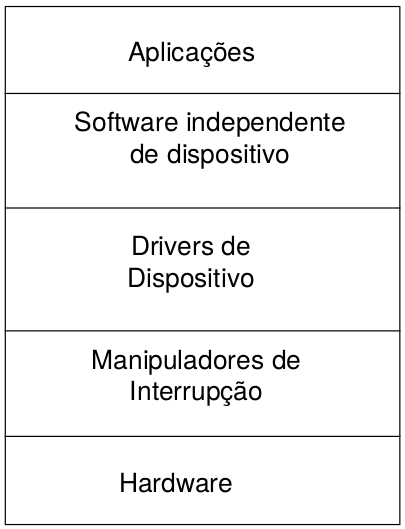
\includegraphics[width=0.35\textwidth]{es-layers}
  \caption{Camadas envolvidas em esquemas de entrada e saída. As camadas 2 à 4 são responsáveis pela gerência de E/S}
  \label{fig:es-layers}
\end{figure}

	\chapter{Sistemas de Arquivos}
Em um computador, os dados podem ser armazenados em vários dispositivos físicos diferentes como disco flexível, fita, disco rígido, CD, etc.. Para simplificar o tratamento, o SO fornece uma visão lógica e uniforme do sistema de armazenamento e uma visão lógica do armazenamento em si, sendo ela o arquivo.

O sistema de arquivo será o módulo do SO responsável pela criação da abstração de arquivos e por seu gerenciamento.

\section{Arquivos}

\begin{definicao}{Arquivo}
  Coleção de dados relacionados entre si
\end{definicao}

Cada arquivo possui um nome, que o identifica. Além do nome, o arquivo possui outros atributos como tipo, nome do criados, tamanho, etc.. As informações contidas em um arquivo geralmente são \textbf{persistentes} e armazenadas em dispositivos não-voláteis.

\subsection{Estruturação}
O servidor de arquivos deve implementar a abstração de arquivo arquivo para o restante do sistema. Para tanto, ele deve determinar como o arquivo será estruturado internamente. As estruturas mais comuns são: sequências de \textit{bytes}, sequência de registros e árvore de registros.


\subsection{Tipos}
Cada sistema de arquivos determina os tipos de arquivos suportados por ele. Sistemsa como o Unix ou o DOS suportam os seguintes tipos:

\begin{itemize}
  \item \textbf{Arquivos Regulares:} contém os dados do usuário;
  \item \textbf{Arquivos Diretório:} arquivos utilizados na manutenção do sistema de arquivos;
  \item \textbf{Arquivos Especiais:} arquivos ligados a dispositivos de E/S.
\end{itemize}


\subsection{Atributos}
Além do nome e dos dados, o SO associa a cada arquivo um conjunto de infomações que auxiliam na ferência dos mesmos. Estas informações adicionais são chamadas atributos e estão geralmente contidas na tabela de arquivos. São exemplos de atributos:

\begin{itemize}
  \item \textbf{Proteção}: indica as permissões de acesso ao arquivo;
  \item \textbf{\textit{Password}:} senha necessária para o acesso ao arquivo;
  \item \textbf{Criador:} usuário criador do arquivo;
  \item \textbf{\textit{Owner}:} proprietário atual do arquivo;
  \item \textbf{\textit{Flag} de oculto:} impede que o nome do arquivo apareça na lista de arquivos;
  \item \textbf{\textit{Flag} de temporário:} o arquivo é deletado quando o processo que o criou morrer;
  \item \textbf{Tamanho:} tamanho atual do arquivo;
  \item \textbf{Tamanho máximo:} tamanho máximo que o arquivo pode atingir;
  \item Instante da última modificação e da criação;
\end{itemize}





\section{Operações sobre Arquivos}
As operações sobre arquivos geralmente levam em consideração um conjunto de entidades de um sistema de arquivos, sendo elas:

\begin{itemize}
  \item \textbf{Tabela de Arquivos:} possui um entrada para cada arquivo, contendo as informações referentes a cada arquivo;

  \item \textbf{Diretório:} caminho que leva ao arquivo. Ao ser criado, o arquivo é posicionado em um diretório e a tabela de arquivos deste diretório deve conter uma entrada para o novo arquivo;

  \item \textbf{Posição Corrente:} ponteiro que indica qual a posição do arquivo será acessada na próxima vez. As operações de leitura e escrita incrementam o valor da posição corrente do arquivo do número de \textit{bytes} lidos e escritos.
\end{itemize}


Agora definimos as operações sobre os arquivos.

\subsubsection{\textit{Create}}
Operação de criação de um arquivo. Deve-se criar uma entrada para o novo arquivo no diretório especificado. Além disso, deve-se criar uma entrada na tabela de arquivos com o nome do criador, data de criação e permissões de acesso. O arquivo recém-criado não possui dado nenhum.


\subsubsection{\textit{Delete}}
libera o espaço ocupao pelo arquivo, deleta a entrada do diretório que aponta para o arquivo e a entrada do arquivo na tabela de arquivos.


\subsubsection{\textit{Open}}
Antes de ser utilizado, o arquivo precisa ser aberto. Essa chamada traz a entrada da tabela de arquivos referente ao arquivo a ser aberto para a tabela de processos do processo que executou o \textit{open}. Este comando retorna um \textbf{descritor de arquivo}, que será utilizado em todas as operações subsequentes sobre o arquivo.


\subsubsection{\textit{Close}}
Esta operação retira a entrada da tabela de arquivos referente ao arquivo indicado da entrada da tabela de processos do processo. Todos os acessos subsequentes ao descritor e arquivo serão invalidados.


\subsubsection{\textit{Read}}
Para ler um arquivo, o processo deve especificar um descritor válido, a quantidade de dados a serem lidos e um local em memória (\textit{buffer}) onde os dados lidos devem ser colocados. A maioria das operações de leitura começam a partir de uma posição corrente.

\subsubsection{\textit{Write}}
Para escrever dados em um arquivos, o processo deve especificar um descritor válido, um \textit{buffer} local que contenha os dados a serem escritos e o tamanho destes dados. Normalmente, os dados são escritos em um arquivo a partir da posição corrente.

\subsection{Manipulação de Arquivos}
Podemos citar:
\begin{itemize}
  \item Criar arquivo;
  \item Abrir o arquivo;
  \item Ler, escrever, operações de \textit{append} e \textit{seek};
  \item Fechar o arquivo;
  \item Deletar o arquivo.
\end{itemize}










\section{Diretórios}
Diretórios são utilizados para auxiliar a disposição dos arquivos no sistema de arquivos. São estruturas hierárquicas, com uma entrada por arquivo. Cada entrada guarda o nome do arquivo, seus atributos e os endereços do disco onde ele está.







\section{Implementação de Arquivos}
A primeira decisão na implementação de arquivos é como os mesmos serão armazenados em blocos de disco. Para a associação de blocos de disco a arquivos, temos três abordagens: alocação contígua, alocação com lista encadeada e nós-i.





\subsection{Alocação Contígua}
Na criação do arquivo, é reservado um espaço contíguo em disco. Para se guardar os endereços de disco associados aos arquivos, necessita-se apenas do endereço inicial do arquivo no disco e seu tamanho.

Em consequência, essa técnica provê uma recuperação de dados extremamente rápida, pois como os blocos são contíguos, o movimento do braço do disco é mínimo. Além disso, é tem fácil implementação.

Entretanto, este método apresenta um alto grau de fragmentação ao longo do tempo. Explicando: uma vez que os blocos são contíguos, após sucessivas exclusões de arquivos, o disco acaba ficando com diversas lacunas ao longo de seu espaço. Quando o disco for preenchido até o final, o espaço das lacunas pode não se suficiente para acomodar arquivos grandes, resultando em falta de espaço, mesmo que, no total de espaço em branco, haja espaço suficiente. Para mitigar este problema, é necessário fazer defragmentação, que e o processo de relocar todos os blocos no inicio do disco, eliminando as lacunas. Note que tal processo é custoso.



\subsection{Lista Encadeada}
Aqui, os bloco continuam sendo mantidos como uma lista encadeada. Porém, na implementação, o ponteiro é colocado em uma tabela geral de blocos. Assim, cada bloco contém um ponteiro para um próximo bloco e o dado que ele carrega.

Esta técnica mitiga o problema da fragmentação, uma vez que arquivos não precisam ser guardados de forma sequencial. Porém, o acesso aleatório a dados é extremamente lento, uma vez que para ler um bloco qualquer, temos que ler todos os blocos que vem antes dele, dado que eles estão em uma lista encadeada.



\subsection{I-nodos}
Aqui, cada arquivo possui uma pequena tabela denominada de i-nodos, que contém os atributos e os endereços dos blocos físicos alocados ao arquivo. Os primeiros endereços de disco são armazenados no próprio i-nodo, que é transferido do disco para a memória no momento da abertura do arquivo.

Em arquivos maiores, o i-nodo ceontém o endereço de um bloco de disco denominado \textbf{bloco indireto simples}. Este bloco é uma tabela de endereços de blocos de disco, podendo haver indireção em segundo e terceiro níveis.









\section{Desempenho do Sistema de Arquivos}
Em geral, um acesso a disco é muito mais lento do que um acesso à memória principal. Uma maneira simples de aumentar a performance do sistema de arquivos é escrever e ler os dados da memória principal sempre que possível.

Para isso, necessitamos manter uma área de memória armazenará temporariamente os blocos de disco mais utilizados. Como essa filosofia se assemelha à filosofia das \textit{caches} físicas, essa ára de memória chama-se \textbf{\textit{cache} de disco}, ou \textit{buffer cache}.

\begin{figure}[h]
  \centering
  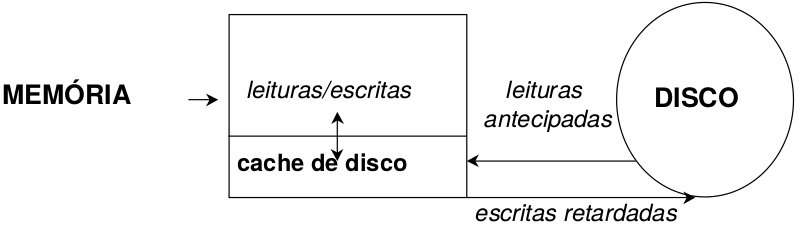
\includegraphics[width=.75\textwidth]{buffer-cache}
  \caption{Esquema geral de \textit{cache} de disco}
  \label{fig:buffer-cache}
\end{figure}

A gerência da \textit{cache} de disco necessita prever o que fazer quando a área reservada para a \textit{cache} estiver cheia. Da mesma maneira que um sistema paginado, devemos escolher um bloco para ser retirado da \textit{cache} de disco. Este problema, apesar de ser parecido com o da substituição de páginas, não deve ser resolvido da mesma maneira.

Além disso, A introdução da \textit{cache} de disco introduz um complicante na área de confiabilidade do sistema. Geralmente , uma operação de escrita em arquivo que retorna sucesso indica que o dado foi escrito no disco com sucesso. Em um sistema com \textit{cache} de disco, isso não é verdade, dado que este retorno simplesmente indica que o dado foi escrito na \textit{cache} de disco com sucesso. Logo, dados assumidos pelo usuário como escritos em disco podem ser perdidos após uma pane do sistema, por estarem em memória apenas.

Este problema se agrava quando os blocos alterados contém estruturas de controle do sistema de arquivos. Assim geralmente, os blocos são divididos em \textbf{blocos críticos} e \textbf{blocos de dados}. Os blocos críticos são sempre escritos na \textit{cache} de disco e no disco, gerando um \textit{bypass} da cache.

\begin{figure}[h]
  \centering
  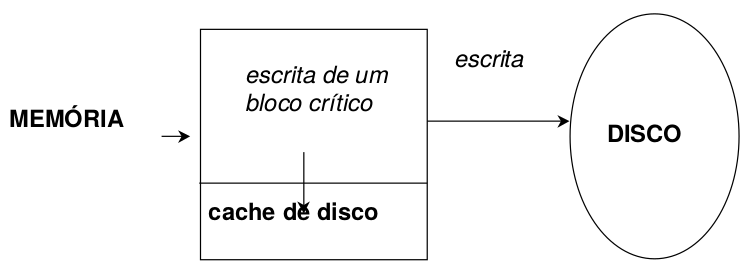
\includegraphics[width=0.75\textwidth]{buffer-cache-critic}
  \caption{\textit{Bypass} na escrita de blocos críticos}
  \label{fig:buffer-cache-critic}
\end{figure}

	\nocite{*}

	% References
	\bibliographystyle{plain} % Plain referencing style
	\bibliography{references} % Use the example bibliography file sample.bib
\end{document}
